% Pages in Thesis should have one of standard U.S. Paper Sizes
% U.S Letter Paper (8.5 x 11) is used.
% Body should be either 11 pt or 12 pt type.
\documentclass[12pt, letterpaper]{thesis}

\usepackage{hyperref}
\usepackage[sorting=debug]{biblatex}
\usepackage{afterpage}
\addbibresource{references.bib}
% For mathematical symbols such as degree
\usepackage{textcomp}
\usepackage{gensymb}
\usepackage{booktabs}

\date{}
\begin{document}

% Front Matter
% Except for the "Abstract" page, every page of thesis must be assigned a
% page number. Placement of consistent page numbers is necessary, and they
% must either be at center, or at the top-right corner.
% Page numbering should be roman numerals for the front matter, and numbered
% for main text.
% Hide page numbers for this page.
\thispagestyle{empty}
\newgeometry{top=1.75in, left=1.5in, right=1in, bottom=1in}
\begin{center}
    EXPLORING THE LIMITS OF ZERO-SHOT LEARNING - HOW LOW CAN YOU GO ?
    
    by
    
    HEMANTH DANDU
    
    (Under the Direction of Suchendra Bhandarkar)
    
    ABSTRACT
\end{center}
Zero-shot learning aims to classify input data into categories with zero training examples. The classification is performed by inferring unseen categories using visual data of seen categories and their relationships with unseen categories. Relationships are determined by using auxiliary data pertaining to categories such as attributes and semantics. Standard zero-shot learning techniques use a large number of seen categories to predict very few unseen categories while maintaining unified data splits and evaluation metrics. This has enabled the research community to advance notably towards formulating a standard benchmark zero-shot learning algorithm. However, the most substantial impact of zero-shot learning lies in enabling the prediction of a large number of unseen categories from very few seen categories within a specific domain. This permits the collection of training data for only a few previously seen categories, thereby mitigating the training data collection process significantly. In this thesis, we focus on the difficult problem of predicting a large number of unseen object categories from very few previously seen categories. We propose a framework that enables us to examine the limits of inferring several unseen object categories from very few previously seen object categories, i.e., the limits of zero-shot learning. In particular, we examine the functional dependence of the classification accuracy of unseen object classes on the number of previously seen classes. We also determine the minimum number of previously seen classes required to achieve pre-specified classification accuracy for the unseen classes on three standard zero-shot learning data sets, i.e., AWA2, CUB and SUN. Additionally, we compare the proposed framework with a prominent zero-shot learning technique on the aforementioned data sets and find that we achieve 21\% higher accuracy on the AWA2 data set, 6\% higher accuracy on the CUB data set, and comparable performance on the SUN data set while providing valuable insights into the unseen class inference process.

%\vspace{2\baselineskip}
\noindent
INDEX WORDS: machine learning, image classification, zero-shot learning, transfer learning

\newpage
\pagenumbering{roman}
% Hide page numbers for this page.
\thispagestyle{empty}
\newgeometry{top=1.75in, left=1.5in, right=1in, bottom=1in}
\begin{center}
    AN EXPLORATION OF MACHINE LEARNING BASED DAY-AHEAD SOLAR IRRADIANCE FORECASTING METHODOLOGIES
    
    \vspace*{2\baselineskip}
    by

    \vspace*{2\baselineskip}
    AASHISH YADAVALLY
    
    B.Tech., Indian Institute of Information Technology Vadodara, INDIA, 2018
    \vspace*{4\baselineskip}

    A Thesis Submitted to the Graduate Faculty of The University of Georgia
    in Partial Fulfillment of the Requirements for the Degree
    \vspace*{3\baselineskip}

    MASTER OF SCIENCE
    \vspace*{3\baselineskip}

    ATHENS, GEORGIA
    
    2020
\end{center}

\newpage
% Hide page numbers for this page.
\thispagestyle{empty}

\begin{center}
    \vspace*{18\baselineskip}
    \textcopyright \hspace{0.05cm} 2020
    
    Hemanth Dandu
    
    All Rights Reserved
\end{center}

\newpage
% Hide page numbers for this page.
\thispagestyle{empty}
\newgeometry{top=1.75in, left=1.5in, right=1in, bottom=1in}
\begin{center}
    EXPLORING THE LIMITS OF ZERO-SHOT LEARNING - HOW LOW CAN YOU GO ?
    
    \vspace*{1\baselineskip}
    by
    \vspace*{1\baselineskip}

    HEMANTH DANDU
\end{center}

\vspace*{6\baselineskip}

\iffalse
\begin{flushright}
Major Professor: $\hskip 0.5em$ Suchendra Bhandarkar
\vspace{\baselineskip}

Committee: \hspace{12pt} $\hskip 2.25em$ Khaled Rasheed \hspace{12pt}\\
Frederick Maier  \\
Karan Sharma  
\end{flushright}
\fi

\begin{flushright}
  \begin{tabular}{ll}
 Major Professor: &Suchendra Bhandarkar \\  [10pt]
    Committee: &Khaled Rasheed \\
    &Frederick Maier \\
    &Karan Sharma \\
  \end{tabular}
\end{flushright}
\vspace*{3cm}


\vspace{3\baselineskip}
\noindent
Electronic Version Approved:\\
Ron Walcott\\
Dean of the Graduate School\\
The University of Georgia\\
December 2020
\newpage
\chapter{1}{Acknowledgements}{Acknowledgements}
\par I would like to thank all my committee members for their time and the numerous suggestions they provided throughout my research. In particular, I would like to thank Dr. Maier for his guidance, constant encouragement and motivation to keep me going. I owe a great debt to Zachary Jones and Chris Barrick who facilitated my introduction into the project, and whose contributions laid the foundation for my work. I am thankful to my friends and family who kept me sane during these unprecedented times, where the whole world has come to a standstill due to COVID-19. I would like to thank everyone at the \textit{Institute for Artificial Intelligence} who presented me with an opportunity to be a part of this project. I would also like to thank Ms. Tino, whose assistance with the administrative tasks at the university made my life incredibly easy.

\newpage
% Print Table of Contents
\listofchapter
\newpage
% Add List of Tables chapter
\listoftables
% Add List of Tables chapter to Table of Contents
\addcontentsline{chl}{chapter}{~LIST OF TABLES}
\newpage
% Add List of Figures chapter
\listoffigures
% Add List of Figures chapter to Table of Contents
\addcontentsline{chl}{chapter}{~LIST OF FIGURES}
\newpage

% Chapters in Thesis
% Chapter 1: Introduction
\pagenumbering{arabic}
\chapter{}{Introduction}{Introduction}

Advances in deep neural networks have empowered machines to achieve human level classification performance on object recognition tasks. Very powerful and robust visual classifier frameworks have been developed, and will no doubt keep improving. In typical object recognition tasks, it is necessary to establish a certain number of predetermined object categories so that classification accuracy can be improved by collecting as many training image samples as possible for each object category. Many problem domains are faced with a large and growing number of object categories. As a consequence, it is becoming increasingly difficult to collect and annotate training data for each object category. Moreover, these images need to capture different aspects of the objects under various imaging conditions to account for the natural variance in appearance for each object category. The problem thus lies in collecting and annotating training data in an efficient and reliable manner for a wide variety of object categories. In addition, trained classifiers can only classify observed object instances into the classes or categories covered by the training data; they lack the ability to deal with previously unseen classes. To address this issue, zero-shot learning (ZSL) techniques have been proposed in the research literature. ZSL frameworks are designed to  tackle the problem of learning classifiers when no explicit visual training examples are provided.

\par
\medskip

Human beings perform ZSL naturally, enabling recognition of at least 30,000 object classes~\cite{humanimageunderstanding}. When faced with a new unfamiliar object, we are, after a while, able to state what it resembles: "A New York City hot dog cart, with the large block being the central food storage and cooking area, the rounded part underneath as a wheel, the large arc on the right as a handle, the funnel as an orange juice squeezer and the various vertical pipes as vents or umbrella supports." It is not a good cart, but we can see how it might be related to one~\cite{humanimageunderstanding}. For humans, it is as easy as recognizing a 10-letter word with 3 wrong letters. However, in the case of machines, we need a vast number of training images for each type of cart to learn to adapt to the naturally occurring variations in cart appearances. In humans, the ability to understand natural variations comes from our existing and ever evolving language knowledge base, which enables us to connect unseen categories with seen categories using high-level descriptions.

\par
\medskip

To emulate the ZSL process in machines, previously unseen object categories are recognized by leveraging auxiliary information related to categories. Auxiliary information are derived from external data sources such Wikipedia, WordNet~\cite{wordnet} etc. which make it analogous to the human (natural language) knowledge base. As the auxiliary inputs usually carry semantic information, they constitute a \textit{semantic space}. A typical source of semantic information used in ZSL is \textit{attribute spaces}. Attribute spaces are semantic spaces that are engineered manually for each domain or data set. Attributes are a list of terms that describe various properties of each object class or category. For example, an attribute could be \textit{hair color} with values "black", "brown", "white" etc. The attributes can be either discrete or continuous. Label-embedding spaces are also often used as a source of semantic information, where the word/label representations are obtained by employing information retrieval techniques on large digital text corpora. Examples of widely used label-embedding models include Word2Vec~\cite{w2v}, GloVe~\cite{glove}, and FastText~\cite{fasttext}. Hierarchical information is another source of semantic information that can be derived from a pre-existing ontology such as WordNet \cite{wordnet}. All sources of auxiliary information when combined together comprise the semantic space.

\par
\medskip

In typical ZSL frameworks, a set of previously observed classes is used to train the visual classifier. These classes are termed as \textit{seen classes}. The framework is then evaluated on another set of previously not observed classes termed as \textit{unseen classes}. While training, the classifier has access to auxiliary information of both the seen and unseen classes. A formal definition of the ZSL task is provided in Definition~\ref{def:zsl}. 
Conventional ZSL is restrictive in its formulation since it assumes that the input images at the time of  prediction or inference can only come from the unseen classes. In contrast, generalized ZSL addresses the more general setting where the input images at the time of  prediction or inference can come from both, the seen and unseen classes~\cite{gen-zsl}. Generalized ZSL is formally defined in Definition \ref{def:gzsl}. 

\par
\medskip

\theoremstyle{definition}
\begin{definition}[Conventional Zero-shot Learning]
\label{def:zsl}
Given labelled training instances $X_s$ belonging to seen classes $Y_s$, zero-shot learning aims to learn a classifier that can classify testing instances $X_u$ belonging to the unseen classes $Y_u$
\end{definition}

\par
\medskip

\theoremstyle{definition}
\begin{definition}[Generalised Zero-shot Learning]
\label{def:gzsl}
Given labelled training instances $X_s$ belonging to seen classes $Y_s$, generalised zero-shot learning aims to learn a classifier that can classify testing instances $X_{u \cup s}$ belonging to the classes $Y_u \cup  Y_s$
\end{definition}

\par
\medskip

Several ZSL frameworks have been proposed in the literature, however, all of these frameworks use a proposed split~\cite{gbu} of standard ZSL data sets~\cite{awa,cub,sun} into seen and unseen classes. This split is formulated in to aid uniform research towards finding a universal ZSL framework that outperforms the existing ones. Altogether, the zero-shot learning problem has been formally framed for each standard data set using specific categories as seen classes and the remaining as unseen classes in a race for attaining maximum classification accuracy. Of the total object categories present in each data set, the number of seen classes has always been significantly higher than the number of unseen classes in most ZSL frameworks. For example, the \textit{Animals-with-Attributes} (AWA2) data set~\cite{awa} has a proposed 40:10 seen:unseen class split, the \textit{Caltech-USCD-Birds} (CUB) data set~\cite{cub} has a 150:50 seen:unseen class split, and the large-scale \textit{Scene Understanding} (SUN) database~\cite{sun} has a 645:72 seen:unseen class split. While this formulation has helped to formulate several benchmark approaches to ZSL tasks, we notice that the original intent of mitigating the data collection process has been skirted at a very early stage. Therefore, we aim to infer larger number of unseen object categories using very few seen object categories. We believe this addresses the original problem of obtaining annotated images to a greater extent. 

\par
\medskip

We propose a new framework that helps us to examine the limits of inferring unseen object categories from very few seen object categories, i.e., test the limits of ZSL. We note the functional dependence of the classification accuracy on the number of previously seen classes across the spectrum of the classes on three widely used object classification data sets~\cite{awa,cub,sun}. An important contribution of the proposed approach is its ability to determine the optimal set of representative classes using which one could infer a large number of previously unseen classes with a pre-specified measure of accuracy. We explore intuitive techniques to select a few seen classes which would enable us to predict a larger number of unseen classes. The proposed approach also aids the training data collection process significantly by identifying the key object categories from which the training data collection process can be initiated and determining which object categories to stop at, based on an expected or pre-specified classification accuracy measure for a specific problem. We evaluate the proposed approach in the generalized ZSL setting, thus making it very practical. We present valuable insights into the inference process for general and specific cases where the proposed approach performs exceptionally well, and also for cases where we fail to infer the correct unseen category. We also compare the proposed approach with the well known Attribute Label Embedding (ALE)~\cite{ale} procedure, which has been shown to perform very well on the aforementioned three standard data sets as published in~\cite{gbu}. In comparison to ALE, we observe that the proposed approach achieves 21\% higher accuracy on the AWA2 data set, 6\% higher accuracy on the CUB data set and comparable performance on the SUN data set. We also establish the minimum number of previously seen classes needed to obtain reasonable (or above average) generalized ZSL performance on the AWA2 data set as 20 seen classes out of a total of 50 classes, on the CUB data set as 80 seen classes out of a total of 200 classes and on the SUN data set as 360 seen classes out of a total of 717 classes.

\par
\medskip

This thesis is organized into six chapters. Chapter 1 introduces the concept of zero-shot learning (ZSL) and summarizes the work done in this thesis. Chapter 2 reviews the related work in ZSL and position our work in the overall ZSL research literature. Chapter 3 describes the various data sets used for experiments carried out in this thesis. Chapter 4 discusses the overall methodology underlying the proposed approach and also explains the finer details about the methods used. Chapter 5 presents the experimental results of the proposed approach on the aforementioned three data sets. Chapter 5 compares the proposed approach with the Attribute Label Embedding (ALE) scheme and shows how well the proposed approach fares in comparison to the widely used ALE-based ZSL framework. Finally, in Chapter 6, we conclude this thesis and discuss directions for future work.
% Chapter 2: Related Work
\chapter{}{Literature Review}{Literature Review}

Zero-shot learning (ZSL) approaches can be broadly classified into two categories based on the unseen class information the model has during the training process. In the inductive ZSL framework, we have access to to labeled image data from the seen classes as well as auxiliary information (i.e., semantic attributes/descriptions) about both, seen and unseen classes during the training phase. In the transductive ZSL framework, we have access to auxiliary information (i.e., semantic attributes/descriptions) about both, seen and unseen classes during the training phase as in the case of the inductive ZSL framework. The major difference is that in the case of transductive ZSL, we have access to labeled image data from the seen classes \textit{and} unlabeled image data from the unseen classes during the training phase which is a departure from inductive ZSL. Within both frameworks, one can make an distinction based on the type of setting used to evaluate the model during testing. i.e. the conventional ZSL setting and generalized ZSL setting as described in Chapter 1. In this section we review work on both the inductive and transductive ZSL frameworks and place the proposed approach within the ZSL taxonomy.

\par
\medskip

Preliminary work in inductive ZSL uses a two-stage approach to infer unseen class labels. In the first stage, the attributes of an image are predicted. In the next stage, the class label is inferred by searching for the class label with the most similar set of attributes. Lampert et al~\cite{DAP} introduced the Directed Attribute Prediction (DAP) and Indirect Attribute Prediction (IAP) models  which use the aforementioned two-stage approach. In DAP~\cite{DAP}, a probabilistic attribute classifier is first learned. The class posteriors are then computed and class labels predicted via a maximum a posteriori (MAP) estimate. In IAP~\cite{DAP}, a multi-class classifier is first used to predict the class posterior. The probability of each class is then used to compute the attribute posteriors of an image. While the DAP and IAP frameworks have historically been some of the most widely cited ZSL methods in the literature, they suffer from the problem of domain shift~\cite{domainshift} where the intermediate functions learned from the auxiliary information without any adaptation to the target domain introduce an unknown bias.

\par
\medskip

Subsequent ZSL frameworks attempt to learn a compatibility function from image feature space to the semantic or auxiliary space. These frameworks can be further categorized based on the type of compatibility function that they learn. The first set of methods learn linear compatibility functions whereas the next set of methods learn non-linear compatibility functions.

\par
\medskip

\noindent
\textbf{Linear Compatibility.} Attribute Label Embedding (ALE)~\cite{ale} learns a bi-linear compatibility function between the image space and auxiliary space using a weighted approximate ranking objective. ALE improves upon DAP \cite{DAP} significantly since it can use multiple sources of auxiliary information such as word embeddings and class taxonomies. ALE also overcomes the drawbacks of the two-step process used in DAP by directly predicting the class label without the need for an intermediate step. The Deep Visual-Semantic Embedding (DEVISE) model~\cite{devise} also learns a linear mapping between the image space and semantic space and has been shown to perform well on the large-scale ImageNet data set. The Structured Joint Embedding (SJE) scheme~\cite{SJE} uses an unregularized structured SVM to learn the compatibility function coupled with the Stochastic Gradient Descent (SGD) algorithm for optimization. The Embarrassingly Simple Zero-Shot Learning (ESZSL) scheme~\cite{ESZSL} uses an additional regularization term to suppress noise in the auxiliary space. 

\par
\medskip

\noindent
\textbf{Non-Linear Compatibility.}  The Latent Embedding (LATEM) scheme~\cite{LATEM} extends linear compatibility approaches by learning multiple mappings thereby finding a piece-wise linear compatibility function using every image-class pair. LATEM shows improved accuracy over the state-of-art the linear compatibility-based SJE scheme~\cite{SJE}. The Cross-Modal Transfer (CMT) scheme~\cite{CMT} uses a neural network with two hidden layers to learn non-linear projections from image space to Word2Vec~\cite{w2v} space. CMT exploits only information from word embeddings and does not use other sources of auxiliary information such as class attributes used by other methods.
%%% SMB: INCLUDE THE FOLLOWING REFERENCE AND CITATION FOR CMT:
%%% R. Socher, M. Ganjoo, C.D. Manning and A.Y. Ng, Zero-Shot Learning Through Cross-Modal Transfer, Proc. NIPS 2013.  

\par
\medskip

Drawing from linear and non-linear compatibility approaches, hybrid models~\cite{gbu} learn a joint embedding of both the image and semantic features into a combined intermediate space. The Semantic Similarity Embedding (SSE) scheme~\cite{sse} uses a max-margin framework to jointly optimize domain data and semantic data. The Convex Combination of Semantic Embeddings (CONSE) scheme~\cite{conse} is inspired by DEVISE~\cite{devise} and maps images into the semantic embedding space via convex combination of the class label embedding vectors without the need for additional training. Synthesized Classifiers (SYNC) \cite{sync} introduces a set of “phantom” object classes whose coordinates exist in both the semantic space and the model space which are then optimized using labeled data such that the synthesized real object classifiers achieve optimal discriminating performance. Wang et al.~\cite{gcn} use a Graph Convolution Network (GCN) and the GLoVe text embedding model~\cite{glove} to generate a knowledge graph embedding. The knowledge graph embedding exploits both, semantic embeddings and domain relationships to predict the object classifiers. 
%%% SMB: INCLUDE THE FOLLOWING REFERENCE AND CITATION FOR CONSE:
%%% M. Norouzi, T. Mikolov, S. Bengio, Y. Singer, J. Shlens, A. Frome, G.S. Corrado, and J. Dean, Zero-Shot Learning by Convex Combination of Semantic Embeddings, Proc. ICLR, 2014. 

\par
\medskip

Recently, there has been a rise in the use of generative models for ZSL that represent each class as a probability distribution. Generative Framework for Zero-Shot Learning (GFZSL)~\cite{gfzsl} models the class-conditional distributions of seen as well as unseen classes using a multi-variate Gaussian distribution. Generative models such as GFZSL exhibit a significant performance boost in the transductive ZSL setting. The Feature Generating Network (FGN)~\cite{fgn} introduces a novel Generative Adversarial Network (GAN) that synthesizes Convolutional Neural Network (CNN) features conditioned on class-level semantic information, offering a direct shortcut  from a semantic descriptor of a class to a class-conditional feature distribution. The Leveraging the Invariant Side GAN (LisGAN) approach~\cite{LISGAN} generates unseen features from random noise functions which are conditioned by the semantic descriptions. They train a conditional Wasserstein GAN in which the generator synthesizes fake unseen features from noises and the discriminator distinguishes the fake from real via a minimax game. The recent approach based on leveraging the semantic relationships between the seen and unseen object categories termed as LsrGAN~\cite{lsrGAN} performs explicit knowledge transfer by incorporating a novel Semantic Regularized Loss (SR-Loss) function. A Tensorflow-based combination of a Variable Auto-Encoder (VAE) and GAN, termed as TF-vaegan~\cite{tf-vegan}, introduces a feedback loop from a semantic embedding decoder, that iteratively refines the generated features during both the training and feature synthesis stages. The synthesized features together with their corresponding latent embeddings from the decoder are then transformed into discriminative features and exploited during classification to reduce the ambiguities amongst the categories. The TF-vaegan framework~\cite{tf-vegan} is currently regarded as the benchmark in inductive and transductive ZSL settings on the AWA2~\cite{awa}, CUB~\cite{cub}, and SUN~\cite{sun} data sets on the zero-shot learning and generalized zero-shot learning settings. 

\par
\medskip

The proposed framework draws from the two-stage approach used by the DAP and IAP approaches~\cite{DAP} but the problem being addressed is substantially different from the standard ZSL problem that the aforementioned ZSL frameworks are designed for. Note that the proposed approach aims to predict a large number of unseen classes from few seen classes, and consequently, we have far less training data compared to the conventional ZSL settings. Hence, generative-adversarial-based and compatibility learning-based ZSL frameworks which require a lot of training data would be expected to perform poorly in this situation. The proposed ZSL framework represents a first step towards a novel ZSL problem formulation that strives to understand how classification accuracy measures change with change in number and type of seen classes. The proposed framework also allows for selection of an optimal number and type of seen classes based on an expected overall classification accuracy measure which aids in the training data collection process.

\newpage
% Chapter 3: Multi-model Solar Irradiance Forecasting
\chapter{}{{Solar Forecasting Using Numerical Weather Prediction Models}}{Solar Irradiance Forecasting Using Numerical Weather Prediction Models}

\subchapter{Overview}
For a days-ahead forecast horizon, utilizing Numerical Weather Prediction (NWP) models, which predict the evolution of the atmospheric system have been shown to be more useful \cite{thesis_zach}. The NWP models derive their initial conditions from different ground and airborne sensors from across the world. Based on thermodynamic equations describing the physical processes occurring in atmosphere, they forecast different weather variables into the forecast horizon. The National Oceanic and Atmospheric Administration (NOAA) operates a variety of NWP models with their spatial resolution ranging from approximately 10 km - 50 km, and their temporal resolution typically being 1 hour or 3 hours \cite{multimodel_bestpractices}. 

\par Solar forecasting researchers have successfully employed meteorological forecasts from NWP models for forecasting applications for years. The making of a weather forecast involves assessing the current weather situation, assimilating observational information, and projecting this initial state into the future based on the laws of thermodynamics. Weather forecasting employs a set of equations that describe the flow of fluids, being run over a geographic area. Several parameterizations of physical processes are carried out, based on the physical and statistical representations of the physical process. This is useful to approximate the bulk effects of the physical processes.

\par One of the major challenges faced in this process is determining the range of area to observe. The further the forecasting of the weather conditions, i.e, higher the forecast horizon, wider is the range of area that needs to be observed. Multiple weather prediction models, both global and regional, depending on the spatial domain, are maintained by the National Oceanic and Atmospheric Administration (NOAA). Global Forecast System (GFS) is one of the widely-known global weather prediction models, which represents the atmospheric state as a superposition \restoregeometry\noindent of wave functions. It covers the entire globe at a base horizontal resolution of $28km$ between grid points, predicting weather out to $16$ days. Within continental United States, North American Mesoscale (NAM), Rapid Refresh (RAP), High Resolution Rapid Refresh (HRRR) are the popular regional weather prediction models, each having it's own advantages. The NAM Forecast System follows a complex cloud prediction scheme accounting for the internal cloud processes, and thus has better cloud parameterizations over RAP and HRRR. 

\par In this work, we developed machine learning models to forecast solar irradiance on multiple dual-axis tracking (array A), fixed-axis (array B) and single-axis tracking (array E) solar arrays. The irradiance predictions were made 24 hours into the future, at a one-hour temporal resolution. The NAM Forecast System, which can predict parameters describing cloudiness \cite{multimodel_nam}, was input to these predictive models. A weather forecast dataset spanning NAM data for the years 2017 and 2018 was created, though a few forecasts are missing sporadically. 

\par In order to gauge the effect of different weather variables specified by the NAM Forecast System on the solar irradiance predictions, the following were evaluated: air temperature, geopotential height, cloud cover, visibility, wind speed, dew point temperature, air pressure, downward shortwave radiation flux, downward longwave radiation flux, and humidity. Using \textit{random forests}, the more relevant of these weather variables were identified. It was observed that the irradiance readings from the solar farm for each of the arrays were influenced more by the surface temperature, downward short-wave radiation flux, total cloud cover, and atmospheric height. Thus, the remaining weather variables were discarded. This enabled a cut in computational cost of modeling and also led to an improvement in the performance of the models.

\par Each of the weather variables in the NAM Forecast System are projected 36 hours into the future, at a 1-hour temporal resolution. Of these, the effect of the first 24 feature projections on the target solar irradiance was analyzed based on the \textit{mutual information} statistical measure. It was found that the weather variable for a particular target hour offset in the forecast horizon depends on only 6 feature projections following the target hour offset, and 6 feature projections preceding the target hour offset. Separate machine learning models were trained, and the efficacy of the proposed input-selection scheme was tested. 

\par The performance of this input-selection scheme was compared with the methodology followed by Jones \cite{thesis_zach}. It was observed that the input-selection scheme resulted in an average improvement in mean absolute error ($MAE$) across machine learning models by 19.05\%, 19.68\% and 10.65\% for the dual-axis tracking, fixed-axis and single-axis solar arrays respectively. \textit{Random forests} achieved a best performance for such predictive models, with an $MAE$ of 72.63 $W/m^2$, 44.94 $W/m^2$ and 63.60 $W/m^2$ for each of the arrays.

\par The effect of the geographic expansion of weather forecast coverage was analyzed by including the $3$ x $3$ and $5$ x $5$ \textit{geo shapes}, wherein weather forecasts data from eight and twenty four NAM data grid cells centered around the NAM data grid representing Athens, Georgia were incorporated respectively. Such a spatial expansion was assessed for the attribute-selected weather forecast data, obtained by incorporating the input-selection scheme. It was found that the geographic expansion had a detrimental effect on the performance of the machine learning models, and had a marginal improvement with respect to the $1$ x $1$ \textit{geo shape} only for random forests, with the $5$ x $5$ \textit{geo shape} resulting in $MAE$ of 69.38 $W/m^2$, 43.62 $W/m^2$, 61.99 $W/m^2$ for the dual-axis tracking, fixed-axis and single-axis tracking solar arrays respectively.

\subchapter{North American Mesoscale (NAM) Weather Prediction Model}
\par The North American Mesoscale (NAM) Forecast System is based on the Weather Research and Forecasting (WRF) model infrastructure, following non-hydrostatic dynamics and thus enabling vertical momentum estimations. It provides high resolution forecasts over North America for a forecast horizon of 84 hours, the first 36 of which are at a one hour temporal resolution, and the remaining thereafter, at a 3 hour temporal resolution. The forecasts are published for a grid spanning approximately $12km$ x $12 km$ across the continental United States, which are released four times daily at 00h, 06h, 12h and 18h UTC.

\begin{figure}[ht]
    \begin{center}
    	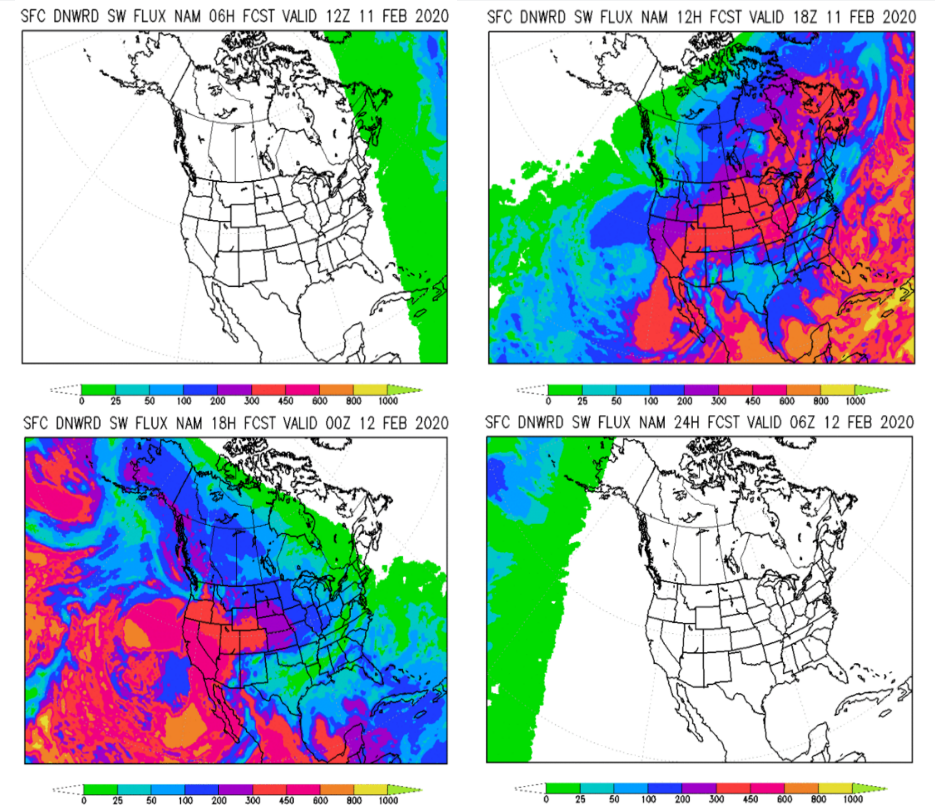
\includegraphics[width=0.85\textwidth]{chapter3/fig_nam_dswrf.png}
    	\caption[Downward shortwave radiation flux parameter for 06h, 12h, 18h, 24h UTC forecasts in a day for NAM Forecast System]{Downward Shortwave Radiation Flux parameter from NAM data over North America domain for 06h forecast (top-left), 12h forecast (top-right), 18h forecast (bottom-left) and 24h forecast (bottom-right) UTC for 11th February, 2020.}
    	\label{fig:fig_nam_dswrf}
    \end{center}
\end{figure}

\par In general, the NWP models cannot realize the  physical phenomenon occurring within an individual grid. Vertical redistribution of heat and moisture can easily occur between mesoscale grids resulting in sub grid-scale variations in convection. The NAM Forecast System repeatedly nudge the temperature and moisture profiles in a grid towards decreasing the convective instability. Moreover, the wider forecast horizon of the NAM Forecast System requires it to model the radiative properties within the clouds effectively \cite{multimodel_rtm}. The NAM models handle this by implementing columnar Radiative Transfer Models (RTMs), which parameterize the cloud properties for every vertical level individually.

\par Dozens of weather variables are available in a NAM model data grid pertaining to environmental components such as altitude, atmospheric pressure, atmospheric radiation, air temperature, water vapour, atmospheric winds, precipitation, soil properties and cloud cover. Each of these are spread across 60 vertical levels in a 0 - 3 km layer, and across 39 pressure levels from 50mb to 1000mb at 25mb intervals. From among these variables, in Fig.~\ref{fig:fig_nam_dswrf}\footnote{NAM forecast snapshots retrieved from: \url{https://www.emc.ncep.noaa.gov/mmb/mmbpll/etapll}}, the averaged \textit{downward short-wave radiation flux} over North America for the four forecasts on 11th February, 2020 is reported.

\subsubchapter{Data Collection}
\subsubsection*{Weather Forecasts}
\par As mentioned in 3.1.1, North American Mesoscale (NAM) Forecast System data was collected from the years 2017 and 2018 for experiments. From this data, surface-level variables as described in Table \ref{Tab:table_nam_variables} were retrieved and analyzed. NAM Forecast System projects different weather parameters 84 hours into the future. The first 36 feature projections in the forecast horizon are at a 1-hour temporal resolution, and subsequent 48 hours of the forecast horizon has feature projections at a 3-hour temporal resolution. In this work, we consider the first 24 feature projections (which are at a 1-hour temporal resolution) for each of the weather variables along with their corresponding target pyranometer readings. 

\begin{table}[h]
\begin{center}
    \caption{NWP-NAM weather variables used in model development}
    \label{Tab:table_nam_variables}
    \begin{tabular}{ c c c}
    	\toprule
    	\textbf{Label} & \textbf{Description} & \textbf{Unit} \\
    	\midrule
    	PRES\_SFC & Air Pressure & $Pa$\\
    	HGT\_SFC & Geopotential Height & $gpm$ \\
    	HGT\_TOA & Height at Planetary Boundary Layer & $gpm$ \\
    	TMP\_SFC & Air Temperature & $K$\\
    	VIS\_SFC & Visibility & $m$\\
    	UGRD\_TOA & U-Component of Wind Speed & $m/s$\\
    	VGRD\_TOA & V-Component of Wind Speed & $m/s$\\
    	DSWRF\_SFC & Downward Short-Wave Radiation Flux & $W/m^2$\\
    	DLWRF\_SFC & Downward Long-Wave Radiation Flux & $W/m^2$\\
    	TCC\_EATM & Total Cloud Cover & $\%$ \\
    	\bottomrule
    \end{tabular}
\end{center}
\end{table}

\subsubsection*{Temporal Features}
\par In this work, temporal features were designed so as to include the \textit{time of day} and \textit{time of year} representations of the forecasts, which incorporate the periodicity in time\footnote{In \cite{thesis_zach}, Jones attempted to use the \textit{time of day} and \textit{time of year} representations by scaling the epoch representing the reference time (in nanoseconds) with the inverse of $8.64e+13$ (number of nanoseconds in a day) and $3.1536e+16$ (number of nanoseconds in a year) respectively, and including their \textit{sine} and \textit{cosine values}. However, these do not appear to be correct as they do not capture the periodicity of the reference time.}. The \textit{time of day} was computed by scaling the number of seconds in the reference time with the inverse of $8.64e+4$ (number of seconds in a day); and the \textit{time of year} was computed by scaling the day of the year with the inverse of $365$ or $366$, depending on whether it is a leap year or not. The sine and cosine values of these measures were added as the temporal features. Such \textit{time of day} representations make the temporal features pertaining to the target hour in the forecast horizon different from that of the reference time. Thus, temporal features representing the target hours in the forecast horizon were also included along with their corresponding predictors.

\subsubsection*{Irradiance Observations}
\par The target irradiance observations are obtained from three solar arrays in the solar farm, namely array A, array B and array E, representing a dual-axis tracking array, fixed axis array with 200$^{\circ}$(SW) azimuth, and a single-axis tracking array respectively. Each of the solar arrays are installed with thermopile pyranometers from different manufacturers such as Kipp \& Zonen\footnote{\url{https://www.kippzonen.com/}}, and LICOR\footnote{\url{https://www.licor.com/}}. The thermopile pyranometers have a black absorptive surface which uniformly absorbs the solar radiation across the short-wave solar spectrum, i.e, between 0.2 $\mu m$ and 3 $\mu m$. 

\begin{figure}[ht]
    \begin{center}
    	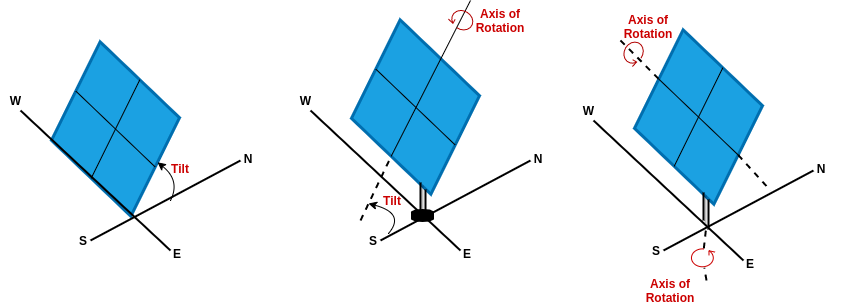
\includegraphics[width=0.85\textwidth]{chapter3/fig_pyranometers.png}
    	\caption[Fixed axis, Single-axis tracking, Dual-axis tracking Solar Arrays]{Fixed axis (left), Single-axis tracking (center), Dual-axis tracking (right) Solar Arrays.}
    	\label{fig:fig_pyranometers}
    \end{center}
\end{figure}

The fixed axis solar array has limited exposure to the sun, owing to the change in position of the sun during the day from morning to night. Thus, the solar radiation captured by this solar array is reduced. Though this limitation is minimized by installing the fixed solar array at an optimized tilt angle, the solar radiation captured by solar tracking arrays is still considerably higher. In order to maximize the overall solar energy captured, it is necessary to ensure that the angle of incidence of the sunlight on the solar array is constantly perpendicular. This is achieved with the help of single-axis trackers (horizontal and vertical), which have one degree of freedom acting as an axis of rotation; and dual-axis trackers which have two degrees of freedom acting as axes of rotation normal to one another \cite{irradiance_solartracker}. This ability to move along the axes enhances the morning and afternoon performance of the solar tracking systems.

\par While the irradiance observations from the solar arrays are received every five seconds, the NWP NAM model data is available only for four reference times in a day, i.e 00h, 06h, 12h, 18h UTC through 2017 and 2018. Thus, for the target hours in the forecast horizon of all the reference times in 2017 and 2018, for which the NWP NAM model data was collected, the irradiance observations were sampled. In Fig.~\ref{fig:fig_average_irradiance}, the average monthly solar radiation captured by the dual-axis tracking, fixed-axis and single-axis tracking solar arrays through 2017 is shown. It can be observed that the solar radiation captured by the tracking arrays (dual-axis and single-axis) is consistently higher than that captured by the fixed axis array.

\begin{figure}[ht]
    \begin{center}
    	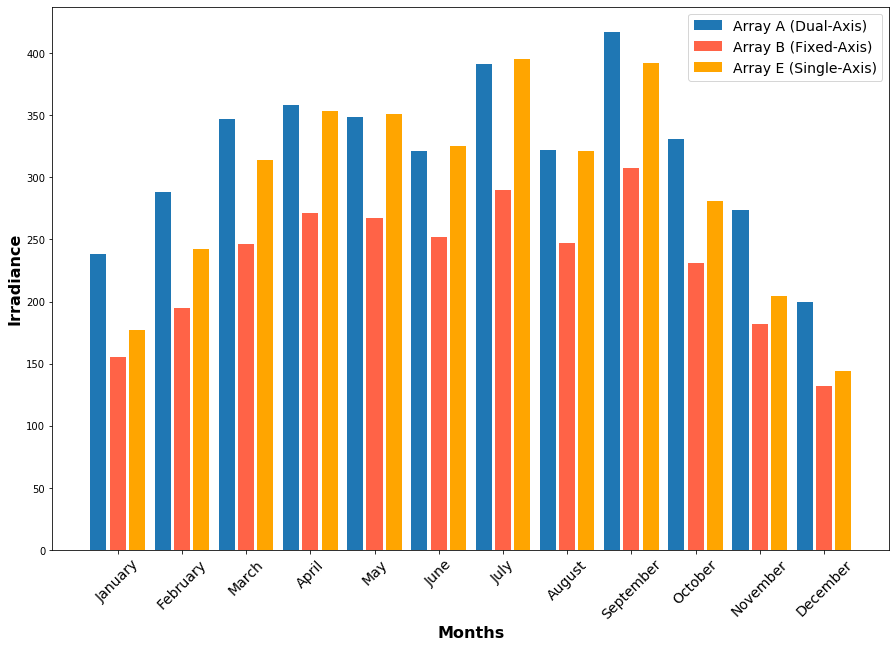
\includegraphics[width=0.85\textwidth]{chapter3/fig_average_irradiance.png}
    	\caption[Average monthly solar radiation captured by dual-axis tracking, fixed-axis and single-axis tracking solar arrays through 2017.]{Average monthly solar radiation captured by dual-axis tracking, fixed-axis and single-axis tracking solar arrays through 2017.}
    	\label{fig:fig_average_irradiance}
    \end{center}
\end{figure}

\subsubchapter{Evaluating Impact of Weather Variables on Irradiance Observations}
\par Mutual information is the measure between two possibly multi-dimensional variables, which quantifies the amount of information obtained from one variable about the other. The relationship detected between the variables can involve either mean, variance or even the higher moments \cite{feature_selection_mi}. The most straightforward and widespread approach towards estimating mutual information follows partitioning the supports of $X$ and $Y$ into bins of finite size, and approximating the sum in the following way:
\begin{equation}\label{eq:eq_mi}
I(X, Y) \approx I_{binned}(X, Y) \equiv \sum_{ij} p(i, j) . log(\frac{p(i, j)}{p_x(i).p_y(j)})
\end{equation}

\par In this work, the mutual information measure was estimated using the \textit{scikit-learn}\footnote{\url{https://scikit-learn.org/stable/}} machine learning software, which makes use of a non-parametric method based on entropy estimation from the \textit{k-nearest neighbors} as described in \cite{feature_selection_mi} and \cite{feature_selection_mi2}. Mutual information measure was calculated for different weather variables from the NAM data and corresponding irradiance observations from the solar arrays as described in the previous subsections. From among the weather variables, it was observed that downward shortwave radiation flux, air temperature, height at planetary boundary layer and total cloud cover have a mutual information score greater than 0.1, indicating a relatively higher dependency on the irradiance observations.

\par Downward shortwave radiation flux is the total amount of shortwave radiation that reaches the earth's surface, and is a major component of the total solar radiation on the surface of the earth. Thus, it is the most direct parameter in the estimation solar irradiance, and the high mutual information score between this weather variable and the irradiance observations from the solar farm is understandable. By absorbing the incoming solar radiation, the Earth warms up, and its temperature rises. As long as the amount of incoming radiative flux is greater than the outgoing radiative flux, the Earth will continue to warm. Thus, the air temperature at the surface is essential in estimating the amount of heat absorbed at that particular location, which in turn reveals information about the amount of solar radiation absorbed by the thermopiles in the pyranometers. 

\par The influence of clouds on solar irradiance is significant. In the absence of visible clouds, aerosols, precipitable water and other atmospheric conditions affect the transmission of solar radiation through atmosphere. In cloudy conditions though, the clouds absorb a significant amount of the shortwave radiation, making variables like total cloud cover, which is the fraction of the sky covered by visible clouds essential. The planetary boundary layer (PBL) is the lowest part of the atmosphere which is directly influenced by its contact with the planetary surface. The structure of turbulence within this layer is mainly governed by the PBL height, which is higher during the day, and lower and more stable during nighttime \cite{feature_selection_pbl1}. PBL height characterizes the planetary boundary layer in a fairly integrated manner and affects the weather parameters such as cloud cover and heat flux \cite{feature_selection_pbl2}. This makes PBL height an important parameter in predicting solar irradiance.

\par For the machine learning models to be able to capture and reconstruct the underlying relationship between input-output data pairs effectively, input selection is essential. By removing the redundant and misleading data, input selection often helps in reducing the computational costs, and improves the accuracy. Several approaches have been defined in literature for the purpose of input selection. In addition to assessing the mutual information scores, we used \textit{random forests} to identify the more important weather variables, as they provide an in-built feature selection.

\par Random forests employ tree-based strategies, which naturally rank inputs based on how well they improve the purity of the node. They are an ensemble learning technique constructed over a variety of randomized decision trees, each of which is built over a random extraction of features and data observations. The training of these randomized decision trees is done with the objective of decreasing the \textit{Gini Impurity}, and the features which help in decreasing this measure are selected \cite{feature_selection_rf}. Thus, random forests help determine the importance of the features in this manner. It was observed that the weather parameters with higher mutual information scores also received high feature importance scores through this technique, thus validating the dependence of the target irradiance observations on this set of parameters.

\par In \cite{thesis_zach}, Jones used 37 weather attributes, of which one corresponds to the weather data at the reference time and 36 are feature projections at an one-hour temporal resolution in the forecast horizon, as the predictor variables for machine learning models. In this work, a forecast horizon of 24 hours was selected, and the relationship between the weather attributes in this forecast horizon and the irradiance observations corresponding to the target hours in this forecast horizon was studied. 

\begin{figure}[htb]
    \begin{center}
    	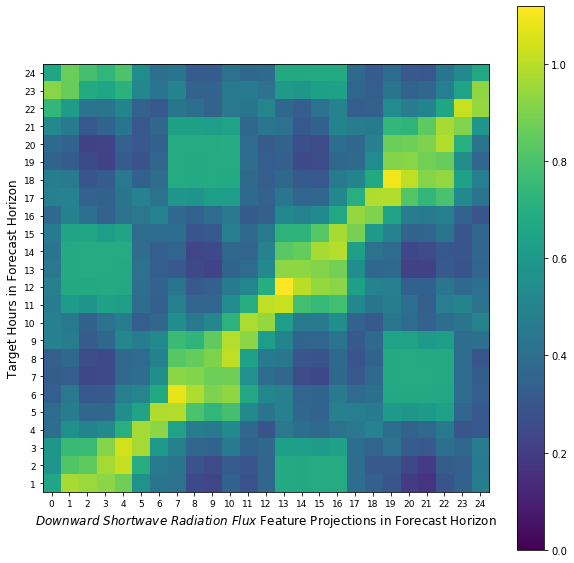
\includegraphics[width=0.65\textwidth]{chapter3/fig_mi_forecast_target.png}
    	\caption[Mutual information between Downward Shortwave Radiation Flux feature projections in forecast horizon and irradiance observations for corresponding target hours from fixed-axis solar array]{Mutual information between feature projections of Downward Shortwave Radiation Flux in the forecast horizon and irradiance observations for corresponding target hours along fixed-axis solar array.}
    	\label{fig:fig_mi_forecast_target}
    \end{center}
\end{figure}

\par As was noted earlier, downward shortwave radiation flux was the most important NAM weather variable with respect to the irradiance observations in the solar farm. In Fig.~\ref{fig:fig_mi_forecast_target}, the mutual information between the feature projections of this weather variable and the corresponding irradiance observations from fixed-axis solar array are represented in a heatmap, wherein, different colours in the colour-bar depict the amount of mutual information measure. It can be observed that the irradiance observations from fixed axis array for a particular target hour are relatively more dependent on only a certain number of feature projections in the forecast horizon. Thus, for the machine learning models trained for each target hour in the forecast horizon, feature projections from six hours ahead, and six hours prior were considered as predictors. 
\par For the first six target hours in the forecast horizon which do not necessarily have six prior feature projections, desired number of feature projections were selected from the end. Similarly, for the last six target hours in the forecast horizon which do not necessarily have six subsequent feature projections, desired number of feature projections were selected from the beginning of the forecast horizon. Such a feature projection selection is justified because it is more likely for the same reference time in two consecutive days to have similar weather conditions. Thus, following this input selections scheme, the NAM model data contributes 13 feature projections for each of the four environmental attributes described earlier, eight temporal features (four for the reference time of the forecast, four for the target hour offset from the reference time) towards the post-processing of solar irradiance from each of the solar arrays using machine learning models.

\subchapter{Experiment Setup}
\par In this chapter, two series of experiments are performed towards predicting solar irradiance on the dual-axis tracking, fixed-axis and single-axis tracking solar arrays. In the first series of experiments, solar irradiance forecasting using Numerical Weather Prediction (NWP) models such as North American Mesoscale (NAM) Forecast System is investigated, replicating the modeling methodology employed by Jones in \cite{thesis_zach}. This is compared with the processed NAM dataset obtained by incorporating the input selection scheme described in 3.2.2. 

\par In this work, 24-hour \textit{persistence models} were used to set a baseline for the more sophisticated machine learning models. Based on the assumption that conditions remain unchanged between the current time and a future time, 24-hour \textit{persistence models} measure the solar irradiance at a particular time $t$ based on the irradiance measured at $t-24$. Making use of such a trivial model as baseline provides a reference for improving the machine learning models. 

\par Several machine learning algorithms such as \textit{Least-Squares Linear Regression} (LSLR), \textit{k-Nearest Neighbors} (KNN), \textit{Support Vector Regression} (SVR), \textit{Decision Trees} (DT), \textit{Random Forests} (RF) and \textit{Extreme Gradient Boosted Trees} (XGBT) were used for the purpose of forecasting. Python-based machine learning softwares \textit{scikit-learn} and \textit{xgboost}\footnote{\url{https://github.com/dmlc/xgboost}} were used for the implementations of these machine learning algorithms. Randomized cross-validated grid search was employed to identify the optimal set of hyperparameters, ranges for each of which were selected around the default values set for them in the \textit{scikit-learn} implementations.

\par Weather variables from the NAM Forecast System were used as predictors for the machine learning models, and the irradiance observations from the solar arrays were used as target variables. Each of the weather variables are projected 36 hours into the future at a one-hour temporal resolution. As a part of the input-selection scheme, select feature projections were picked from the important weather variables, depending on the target hour in the forecast horizon. Prediction of target irradiance was done for a day-ahead forecast horizon, i.e, solar irradiance was predicted 24 hours into the future at a one hour temporal resolution. Models were trained on data collected during 2017, and evaluated against data collected during 2018. In the first series of experiments, the performance of the models, with and without employing the input-selection scheme was compared.

\par Jones \cite{thesis_zach} reported evaluation metrics such as \textit{mean absolute error} ($MAE$) and \textit{coefficient of determination} ($R^2$). $MAE$ is a more natural and unambiguous measure of average error, and is extremely useful in evaluating average-model performance. An evaluation metric such as $R^2$ helps in providing a reference point for comparing the model results with results from other literature. Owing to these advantages, in this work, both the evaluation metrics were retained to facilitate a consistent comparison. In addition, the correlation coefficient ($r$) is reported as well.

\par Model results were analyzed in two schemes: mean of the evaluations for each forecast hour in the forecast horizon ($Overall$); mean of the evaluations for sets of six forecast hours in the forecast horizon, i.e, $1 - 6$, $7 - 12$, $13 - 18$ and $19 - 24$. $MAE$ was estimated for each of these forecast horizon segments by taking an average of the metric across each of the target hours in the segment. However, for $R^2$ and $r$, this was performed by flattening the predictions and ground-truth values for multiple target hours in the forecast horizon segment into single lists, and computing the metrics over these lists. Such an analysis helped in realizing the performance of the models specifically for different periods in the day. 

\par Geographic expansion of forecast coverage by including additional weather forecasts specific to areas surrounding the target location is considered to improve the solar irradiance forecasting capabilities. In the second series of experiments, the effect of such a spatial expansion is investigated, by including the feature projections of weather variables from a grid of cells around the NAM data grid representing Athens, as predictors to the machine learning models. A geographic expansion from the $1$ x $1$ grid to other \textit{geo shapes} such as $3$ x $3$ and $5$ x $5$ is investigated for the \textit{K-Nearest Neighbors}, \textit{Random Forests} and \textit{Extreme Gradient Boosted Trees} algorithms. Each of these methodologies are further explained in finer detail.

\subsubchapter{Irradiance Forecasting with NAM Forecast System}
\par For the replication study, North American Mesoscale (NAM) weather forecast data and target irradiance data from the solar farm at the University of Georgia were collected for the years 2017 and 2018. For a forecast horizon of 24 hours, planar surface features from the NAM Forecast System such as air pressure, geopotential height, height at planetary boundary layer, air temperature, u-component of wind speed, v-component of wind speed, downward short-wave radiation flux and downward long-wave radiation flux were used. 

\par As mentioned in 3.2.2, it was determined that weather variables such as air temperature, total cloud cover, atmospheric height and downward short-wave radiation flux from among the surface-level planar features affected the solar irradiance predictions more. Hence, the other weather variables were omitted. Depending on the target hour offset in the forecast horizon, select feature projections were picked for the weather variables, so as to be included in the NAM dataset. This was done by selecting 13 from among the 37 weather attributes at a one-hour temporal resolution such that, six followed the reference time of the target hour offset, six preceded the reference time of the target hour offset, and one corresponded to the reference time of the target hour offset. In order to choose an ideal set of parameters for the machine learning models, \textit{hyperparameter tuning} was performed with the help of a randomized cross-validated grid search. 

\par The weather forecast data obtained by both methodologies was input to several machine learning models, which were trained on data collected during 2017, and evaluated against data collected during 2018. The results obtained by both methodologies, i.e with and without incorporating the input selection scheme, were compared and analyzed.

\vspace{0.5cm}

\subsubchapter{Geographic Expansion of Forecast Coverage}
\par Lorenz et al. \cite{expansion_lorenz} found that expanding the forecast region to approximately $100 km$ x $100 km$ resulted in an improvement in day-ahead solar forecasting. They performed a spatial averaging across the region, by taking  an arithmetic mean of the weather variables from the surrounding weather data grid cells. In contrast, Sanders et. al. \cite{publication_sanders} and Jones \cite{thesis_zach} performed a distance-dependent weighted averaging, by including the weather variables from the surrounding weather data grid cells as predictors to the machine learning models.

\begin{figure}[ht]
    \begin{center}
    	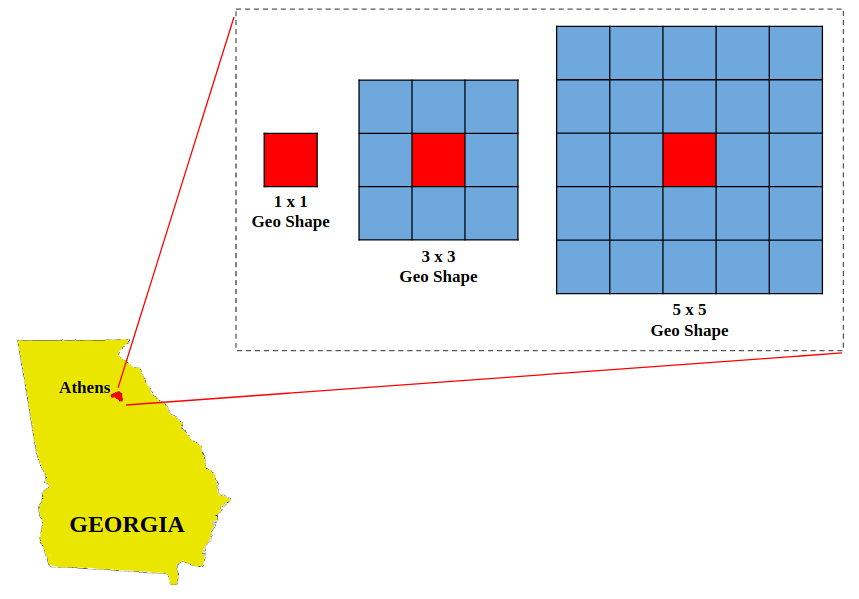
\includegraphics[scale=0.23]{chapter3/fig_geoshapes.png}
    	\caption[Geographic expansion of forecast coverage around Athens NAM model data grid]{Geographic expansion of forecast coverage with 1 x 1 Geo Shape representing Athens NAM model data grid, 3 x 3 Geo Shape and 5 x 5 Geo Shape representing grid of cells around Athens.}
    	\label{fig:fig_geoshapes}
    \end{center}
\end{figure}

\par Jones \cite{thesis_zach} trained \textit{k-nearest neighbors} and \textit{random forest} algorithms for $3$ x $3$, $5$ x $5$ and $7$ x $7$ \textit{geo shapes}, each reflecting a spatial expansion up to $36km$ x $36km$, $60km$ x $60km$ and $84km$ x $84km$ respectively. As shown in Figure~\ref{fig:fig_geoshapes}, each of the \textit{geo shapes} represent eight, fifteen and forty eight NAM weather forecast data grid cells centered around Athens, Georgia. They realized that including the weather forecasts from the surrounding data grid cells resulted in an improved day-ahead solar forecasting, though it was observed that the improvement diminished as the \textit{geo shape} grew larger. Additionally, Jones \cite{thesis_zach} also noted that the $3$ x $3$ \textit{geo shape}, equivalent to a $36km$ x $36km$ area was optimal. 

\par In this work both the schemes were compared: one in which GHI from the surrounding grids is averaged, and other in which weather variables from surrounding cells are included as predictors. It was observed that the latter helped in improving the performance of the models more. Thus, a geographic expansion of weather forecast coverage was carried out with $3$ x $3$ and $5$ x $5$ \textit{geo shapes}, resulting in a spatial expansion upto $60km$ x $60km$. The dataset set up using the input selection scheme described in 3.2.2, was used to determine the effect of geographic expansion.

\vspace{0.3cm}
\subchapter{Results and Discussion}
\subsubsection*{Assessment of Model Performance with and without Input Selection Scheme}
\par In this work, an input selection scheme as described in 3.2.2 was incorporated towards selecting features for the machine learning models. The performance of the machine learning models using both the methodologies, i.e. with and without the input selection scheme were compared for dual-axis tracking solar array, fixed-axis solar array and single-axis tracking solar array. As a part of this scheme, the key differences between Jones' dataset and the one used in this work, towards training with the machine learning models are as follows:
\begin{itemize}
    \itemsep0em
    \item Jones \cite{thesis_zach} hadn't considered the \textit{total cloud cover} weather variable in the NAM weather dataset
    \item from among the other surface-level NAM weather variables used, only air temperature, height at planetary boundary layer and downward shortwave radiation flux were considered
    \item instead of the 37 weather attributes for each of the weather variables, select feature projections depending on the target hour offset were chosen as predictor variables
    \item $1$ x $1$ \textit{geo shape} was selected instead of $3$ x $3$ (which Jones \cite{thesis_zach} had found to be optimal)
    \item \textit{time of day} and \textit{time of year} encodings were modified to incorporate periodicity of the reference time in a particular day or in a particular year
\end{itemize}

%\par Based on these differences, the two NAM datasets were used as input to different machine learning models. Separate machine learning models were trained for each of the target hour offsets between 1 and 24, and their 

\begin{table}[h]
\begin{center}
        \caption[Comparing performance of machine learning algorithms trained against dual-axis tracking array using NAM Forecast System data, with and without input selection.]{Comparing performance of machine learning algorithms trained against dual-axis tracking array utilizing NAM Forecast System data: (a) without input selection (upper), (b) with input selection (lower)}
%    \vspace{0.2cm}
    \label{Tab:fs_array_a}
    \begin{tabular}{@{}p{5.3em}ccccccccc@{}}
    \toprule
    & \textbf{Metric} & \textbf{Horizon} & \textbf{PER} & \textbf{LSLR} & \textbf{SVR} & \textbf{KNN} & \textbf{DT} & \textbf{RF} & \textbf{XGBT} \\ \cmidrule(l){1-10} 
    \multirow{10}{5em}{Without Input Selection} & \multirow{5}{*}{$MAE$} & $1 - 6$ & 153.32 & 231.00 & 88.38 & 98.73 & 98.34 & 74.38 & 73.03 \\
                                              &                   & $7 - 12$ & 153.91 & 231.06 & 89.83 & 101.77 & 105.17 & 77.14 & 76.97 \\
                                              &                   & $13 - 18$ & 154.16 & 232.15 & 89.08 & 106.56 & 98.31 & 74.43 & 75.64 \\
                                              &                   & $19 - 24$ & 161.43 & 243.04 & 89.88 & 104.15 & 98.19 & 75.02 & 76.69 \\
                                              &                   & $Overall$ & 155.71 & 234.31 & 89.29 & 102.80 & 100.00 & \textbf{75.24} & 75.58 \\ \cmidrule(lr){2-10}
                                              & \multirow{5}{*}{$R^2$} & $1 - 6$ & 0.46 & 0.31 & 0.85 & 0.78 & 0.71 & 0.86 & 0.86 \\
                                              &                   & $7 - 12$ & 0.45 & 0.29 & 0.84 & 0.78 & 0.68 & 0.85 & 0.84 \\
                                              &                   & $13 - 18$ & 0.45 & 0.31 & 0.84 & 0.77 & 0.71 & 0.86 & 0.85 \\
                                              &                   & $19 - 24$ & 0.41 & 0.25 & 0.84 & 0.77 & 0.71 & 0.85 & 0.85 \\
                                              &                   & $Overall$ & 0.44 & 0.29 & 0.84 & 0.77 & 0.70 & 0.85 & 0.85 \\ 
    \midrule
    \multirow{3}{5em}{Relative Imp. in $MAE$ (\%)} & & & & & & & & & \\
    & & $Overall$ & --- & 52.17 & 17.76 & 28.97 & 10.91 & 3.47 & 1.02 \\ 
    & & & & & & & & & \\
    \midrule
    \multirow{10}{5em}{Input Selection}
                                              & \multirow{5}{*}{$MAE$} & $1 - 6$ & 153.32 & 107.08 & 70.63 & 68.54 & 85.74 & 70.21 & 71.65 \\
                                              &                   & $6 - 12$ & 153.91 & 114.52 & 73.82 & 72.35 & 90.57 & 72.92 & 74.6 \\
                                              &                   & $13 - 18$ & 154.16 & 115.03 & 73.34 & 73.12 & 87.65 & 72.6 & 75.77 \\
                                              &                   & $19 - 24$ & 161.43 & 111.68 & 75.93 & 78.04 & 92.39 & 74.78 & 77.23 \\
                                              &                   & $Overall$ & 155.71 & 112.08 & 73.43 & 73.02 & 89.09 & \textbf{72.63} & 74.81 \\ \cmidrule(lr){2-10}
                                              & \multirow{5}{*}{$R^2$} & $1 - 6$ & 0.46 & 0.84 & 0.88 & 0.88 & 0.78 & 0.88 & 0.87 \\
                                              &                   & $7 - 12$ & 0.45 & 0.83 & 0.86 & 0.86 & 0.76 & 0.87 & 0.86 \\
                                              &                   & $13 - 18$ & 0.45 & 0.82 & 0.86 & 0.86 & 0.77 & 0.87 & 0.86 \\
                                              &                   & $19 - 24$ & 0.41 & 0.82 & 0.85 & 0.85 & 0.74 & 0.86 & 0.85 \\
                                              &                   & $Overall$ & 0.44 & 0.83 & 0.86 & 0.86 & 0.76 & 0.87 & 0.86 \\ 
    \bottomrule
    \end{tabular}
\end{center}
\end{table}

\par For the dual-axis tracking solar array, all the machine learning models performed exceedingly well with respect to the baseline 24-hour \textit{persistence} models, which was expected. A substantial improvement was observed for all the machine learning models built using weather forecast data without incorporating the input-selection scheme. In particular, using the input selection scheme helped in improving the $MAE$ of simple \textit{linear regression} by 52.17\%. There was a considerable improvement in the performance of \textit{support vector regression} and \textit{k-nearest neighbors} algorithms as well, with the $MAE$ reducing by 17.76\% and 28.97\% respectively. Each of these algorithms is greatly affected by a higher dimensionality and quality of data, and by weeding out weather variables and their feature projections which have a lesser influence on the target irradiance, the improvement in performance of these models can be justified.   

\par Ensemble tree-based methods have the intrinsic ability to calculate feature importance, and account for the possible correlations between the variables. Thus in general, they perform better than the linear regression methods. For the dual-axis tracking array, random forests had the best performance with an $MAE$ of 72.63 $W/m^2$, and extreme gradient boosted trees recorded an overall $MAE$ of 74.81 $W/m^2$. The improvement over the performance of the same algorithms without incorporating the input selection scheme was 3.47\% and 1.02\% respectively.

\par While the random forests performed the best, considerable improvements in performance as a result of incorporating the input selection scheme were seen in the \textit{support vector regression} and \textit{k-nearest neighbors} algorithms. Overall, there was an average improvement in $MAE$ by 19.05\% across the machine learning models, with \textit{random forests} having the best $MAE$ with 72.63 $W/m^2$ for the dual-axis tracking solar array.

\begin{table}[h]
\begin{center}
    \caption[Comparing performance of machine learning algorithms trained against fixed-axis solar array using NAM Forecast System data, with and without input selection.]{Comparing performance of machine learning algorithms trained against fixed-axis solar array utilizing NAM Forecast System data: (a) without input selection (upper), (b) with input selection (lower)}
%    \vspace{0.2cm}
    \label{Tab:fs_array_b}
    \begin{tabular}{@{}p{5.3em}ccccccccc@{}}
    \toprule
    & \textbf{Metric} & \textbf{Horizon} & \textbf{PER} & \textbf{LSLR} & \textbf{SVR} & \textbf{KNN} & \textbf{DT} & \textbf{RF} & \textbf{XGBT} \\ \cmidrule(l){1-10} 
    \multirow{10}{5em}{Without Input Selection} & \multirow{5}{*}{$MAE$} & $1 - 6$ & 111.23 & 151.79 & 55.018 & 61.10 & 62.81 & 47.09 & 47.21 \\
                                              &                   & $7 - 12$ & 111.51 & 147.12 & 56.65 & 63.78 & 62.05 & 48.32 & 49.56 \\
                                              &                   & $13 - 18$ & 111.97 & 151.09 & 55.64 & 68.70 & 64.64 & 48.19 & 49.22 \\
                                              &                   & $19 - 24$ & 117.15 & 159.29 & 56.11 & 66.53 & 62.28 & 47.65 & 49.44 \\
                                              &                   & $Overall$ & 112.96 & 152.32 & 55.85 & 65.03 & 62.95 & \textbf{47.81} & 48.86 \\ \cmidrule(lr){2-10}
                                              & \multirow{5}{*}{$R^2$} & $1 - 6$ & 0.59 & 0.54 & 0.89 & 0.85 & 0.80 & 0.90 & 0.89 \\
                                              &                   & $7 - 12$ & 0.58 & 0.55 & 0.89 & 0.85 & 0.80 & 0.89 & 0.88 \\
                                              &                   & $13 - 18$ & 0.58 & 0.55 & 0.89 & 0.83 & 0.78 & 0.89 & 0.88 \\
                                              &                   & $19 - 24$ & 0.55 & 0.50 & 0.89 & 0.83 & 0.80 & 0.89 & 0.88 \\
                                              &                   & $Overall$ & 0.58 & 0.54 & 0.89 & 0.84 & 0.80 & 0.89 & 0.88 \\ 
    \midrule
    \multirow{3}{5em}{Relative Imp. in $MAE$ (\%)} & & & & & & & & & \\
    & & $Overall$ & --- & 51.92 & 16.47 & 28.42 & 10.90 & 6.00 & 4.36 \\ 
    & & & & & & & & & \\ 
    \midrule
    \multirow{10}{5em}{Input Selection}
                                              & \multirow{5}{*}{$MAE$} & $1 - 6$ & 111.23 & 69.81 & 44.26 & 42.77 & 55.30 & 42.94 & 44.66 \\
                                              &                   & $6 - 12$ & 111.51 & 74.74 & 47.19 & 46.72 & 55.96 & 45.16 & 46.77 \\
                                              &                   & $13 - 18$ & 111.97 & 79.63 & 47.02 & 47.02 & 56.65 & 45.14 & 46.79 \\
                                              &                   & $19 - 24$ & 117.15 & 68.75 & 48.13 & 49.67 & 56.48 & 46.51 & 48.69 \\
                                              &                   & $Overall$ & 112.96 & 73.24 & 46.65 & 46.55 & 56.09 & \textbf{44.94} & 46.73 \\ \cmidrule(lr){2-10}
                                              & \multirow{5}{*}{$R^2$} & $1 - 6$ & 0.59 & 0.89 & 0.91 & 0.92 & 0.84 & 0.92 & 0.91 \\
                                              &                   & $7 - 12$ & 0.58 & 0.88 & 0.90 & 0.90 & 0.84 & 0.91 & 0.90 \\
                                              &                   & $13 - 18$ & 0.58 & 0.87 & 0.90 & 0.90 & 0.83 & 0.91 & 0.90 \\
                                              &                   & $19 - 24$ & 0.55 & 0.88 & 0.89 & 0.89 & 0.83 & 0.90 & 0.89 \\
                                              &                   & $Overall$ & 0.58 & 0.88 & 0.90 & 0.90 & 0.84 & 0.91 & 0.90 \\ 
    \bottomrule
    \end{tabular}
\end{center}
\end{table}


\par In general, it's expected that the performance of the models degrades as the forecast horizon increases. However, Jones \cite{thesis_zach} did not observe such a pattern, with sometimes, even the $7 - 12$ hour forecast horizon performing worse than $13 - 18$ and $19 - 24$ hours forecast horizons. Such a trend though, was realized in the results obtained by incorporating the input selection scheme. By and large, most of the models displayed a trend where the error increased (performance degraded) with the target hour in the forecast horizon. Considering the overall improvement in performance, it can be inferred that this indicates an improvement in the short-term forecasting ability of the models.

\par Similar trends were also observed in the performance of the machine learning models for irradiance predictions on the fixed-axis solar array (in Table~\ref{Tab:fs_array_b}). The \textit{random forests} performed the best with an $MAE$ of 44.94 $W/m^2$. This model achieved an improvement of 6\% due to the incorporation of the input-selection scheme. In contrast, \textit{random forests}, which were also the best-performing model without incorporating the input-selection methodology (as followed by Jones \cite{thesis_zach}), achieved a $MAE$ of 47.81 $W/m^2$. In all, the input-selection scheme achieved an average improvement of 19.68\% in $MAE$ across all the machine learning models.

\vspace{1em}

\begin{table}[h]
\begin{center}
    \caption[Comparing performance of machine learning algorithms trained against single-axis tracking array using NAM Forecast System data, with and without input selection.]{Comparing performance of machine learning algorithms trained against single-axis tracking solar array utilizing NAM Forecast System data: (a) without input selection (upper), (b) with input selection (lower)}
    \label{Tab:fs_array_e}
%    \vspace{0.2cm}
    \begin{tabular}{@{}p{5.3em}ccccccccc@{}}
    \toprule
    & \textbf{Metric} & \textbf{Horizon} & \textbf{PER} & \textbf{LSLR} & \textbf{SVR} & \textbf{KNN} & \textbf{DT} & \textbf{RF} & \textbf{XGBT} \\ \cmidrule(l){1-10} 
    \multirow{10}{5em}{Without Input Selection} & \multirow{5}{*}{$MAE$} & $1 - 6$ & 128.64 & 174.61 & 67.52 & 83.58 & 77.53 & 56.81 & 57.67 \\
                                              &                   & $7 - 12$ & 128.97 & 176.21 & 70.13 & 86.63 & 82.25 & 60.32 & 61.40 \\
                                              &                   & $13 - 18$ & 129.25 & 176.39 & 68.79 & 91.08 & 81.01 & 58.54 & 60.15 \\
                                              &                   & $19 - 24$ & 135.35 & 182.16 & 68.70 & 87.62 & 82.42 & 58.42 & 60.85 \\
                                              &                   & $Overall$ & 130.55 & 177.34 & 68.79 & 87.23 & 80.80 & \textbf{58.52} & 60.02 \\ \cmidrule(lr){2-10}
                                              & \multirow{5}{*}{$R^2$} & $1 - 6$ & 0.53 & 0.48 & 0.88 & 0.79 & 0.77 & 0.89 & 0.88 \\
                                              &                   & $7 - 12$ & 0.53 & 0.46 & 0.87 & 0.79 & 0.75 & 0.75 & 0.87 \\
                                              &                   & $13 - 18$ & 0.53 & 0.48 & 0.87 & 0.77 & 0.75 & 0.88 & 0.87 \\
                                              &                   & $19 - 24$ & 0.49 & 0.45 & 0.87 & 0.78 & 0.74 & 0.88 & 0.87 \\
                                              &                   & $Overall$ & 0.52 & 0.47 & 0.87 & 0.78 & 0.75 & 0.88 & 0.87 \\ 
    \midrule
    \multirow{3}{5em}{Relative Imp. in $MAE$ (\%)} & & & & & & & & & \\
    & & $Overall$ & --- & 48.39 & 5.9 & 24.65 & 2.08 & -8.68 & -8.46 \\ 
    & & & & & & & & & \\ 
    \midrule
    \multirow{10}{5em}{Input Selection}
                                              & \multirow{5}{*}{$MAE$} & $1 - 6$ & 128.64 & 87.52 & 62.29 & 61.71 & 75.62 & 61.37 & 62.93 \\
                                              &                   & $6 - 12$ & 128.97 & 95.30 & 65.77 & 65.98 & 81.80 & 64.09 & 65.55 \\
                                              &                   & $13 - 18$ & 129.25 & 93.47 & 64.29 & 65.75 & 76.77 & 63.50 & 65.73 \\
                                              &                   & $19 - 24$ & 135.35 & 89.84 & 66.57 & 69.47 & 82.28 & 65.44 & 66.18 \\
                                              &                   & $Overall$ & 130.55 & 91.53 & 64.73 & 65.73 & 79.12 & \textbf{63.60} & 65.10 \\ \cmidrule(lr){2-10}
                                              & \multirow{5}{*}{$R^2$} & $1 - 6$ & 0.53 & 0.86 & 0.88 & 0.88 & 0.80 & 0.89 & 0.88 \\
                                              &                   & $7 - 12$ & 0.53 & 0.85 & 0.87 & 0.86 & 0.77 & 0.87 & 0.87 \\
                                              &                   & $13 - 18$ & 0.53 & 0.85 & 0.87 & 0.86 & 0.79 & 0.88 & 0.87 \\
                                              &                   & $19 - 24$ & 0.49 & 0.85 & 0.86 & 0.86 & 0.77 & 0.87 & 0.87 \\
                                              &                   & $Overall$ & 0.52 & 0.85 & 0.87 & 0.86 & 0.78 & 0.88 & 0.87 \\ 
    \bottomrule
    \end{tabular}
\end{center}
\end{table}

\par In the present investigation of incorporating the input-selection scheme, the most interesting results were seen with the single-axis tracking solar array predictions (in Table~\ref{Tab:fs_array_e}). For the \textit{k-nearest neighbors} algorithm, trends followed the predictions for the other solar arrays reported so far, with a reduction in $MAE$ by 24.65\%. For the predictions with \textit{support vector regression}, a reduction in $MAE$ by 5.9\% was observed. However, this relative improvement in performance was less in magnitude as compared to those observed for dual-axis tracking array predictions and fixed-axis array predictions. In addition, using the tree-based ensemble methods such as \textit{random forests} and \textit{extreme gradient boosted trees}, a degradation in performance was recorded, with the $MAE$ increasing by 8.68\% and 8.46\%. Though \textit{random forests} still performed the best with an $MAE$ of 63.6 $W/m^2$, this performance paled in comparison to that of the \textit{random forests} without incorporating the input-selection scheme, where an $MAE$ of 58.52 $W/m^2$ was obtained. To explain this, the corresponding data and code were investigated. No errors in data processing were found. Moreover, a systematic error would have affected all the arrays, which wasn't the case. 


\subsubsection*{Evaluating Effect of Geographic Expansion of Forecast Coverage}
\par Better performing algorithms in 3.3.1 such as \textit{k-nearest neighbors}, \textit{random forests} and \textit{extreme gradient boosted trees} were retrained on dual-axis tracking, fixed-axis and single-axis tracking solar arrays and corresponding weather forecast data for the year 2017, and evaluated against data belonging to the year 2018. The performance of these models for each of the \textit{geo shapes} $1$ x $1$, $3$ x $3$ and $5$ x $5$ was compared and analyzed.

\par Using the \textit{k-nearest neighbors} algorithm to predict the day-ahead solar irradiance on dual-axis tracking solar array, it was observed that the geographic expansion had a slightly detrimental effect on the performance. Expanding to $3$ x $3$ \textit{geo shape} resulted in increasing the $MAE$ by 1.59\%, and increasing the weather forecast coverage to $5$ x $5$ \textit{geo shape} resulted in increasing the $MAE$ by 0.44\%. For these models, the $1$ x $1$ performed best with a $MAE$ of 73.01 $W/m^2$.

\begin{table}[h]
\begin{center}
    \caption{Evaluating effect of geographic expansion of forecast coverage for dual-axis tracking array.}
    \begin{tabular}{c c c c c c c c c c c}
        \toprule
        \multirow{2}{*}{\textbf{Metric}} & \multirow{2}{*}{\textbf{Horizon}} & \multicolumn{3}{c}{\textbf{KNN}} & \multicolumn{3}{c}{\textbf{RF}} & \multicolumn{3}{c}{\textbf{XGBT}}\\
        \cmidrule{3-11}
         &  & 1x1 & 3x3 & 5x5 & 1x1 & 3x3 & 5x5 & 1x1 & 3x3 & 5x5 \\
        \midrule
        \multirow{5}{*}{$MAE$} & $1 - 6$ & 68.61 & 69.68 & 69.02 & 68.53 & 67.90 & 66.69 & 71.04 & 69.23 & 85.32 \\
        & $7 - 12$ & 72.52 & 73.72 & 72.77 & 72.40 & 71.40 & 69.38 & 73.51 & 72.44 & 87.16 \\
        & $13 - 18$ & 72.86 & 74.27 & 73.06 & 70.82 & 69.85 & 68.39 & 73.69 & 71.91 & 87.47 \\
        & $19 - 24$ & 78.05 & 78.99 & 78.47 & 74.99 & 74.46 & 73.06 & 77.92 & 76.02 & 90.02 \\
        & $Overall$ & \textbf{73.01} & 74.17 & 73.33 & 71.68 & 70.90 & \textbf{69.38} & 74.04 & \textbf{72.40} & 87.49 \\
        \midrule
        \multirow{5}{*}{$R^2$} & $1 - 6$ & 0.88 & 0.87 & 0.87 & 0.88 & 0.88 & 0.89 & 0.87 & 0.88 & 0.84 \\
        & $7 - 12$ & 0.86 & 0.85 & 0.86 & 0.87 & 0.87 & 0.88 & 0.86 & 0.86 & 0.84 \\
        & $13 - 18$ & 0.86 & 0.85 & 0.85 & 0.87 & 0.87 & 0.88 & 0.86 & 0.87 & 0.83 \\
        & $19 - 24$ & 0.85 & 0.84 & 0.84 & 0.86 & 0.86 & 0.87 & 0.84 & 0.85 & 0.83 \\
        & $Overall$ & 0.86 & 0.85 & 0.86 & 0.87 & 0.87 & 0.88 & 0.86 & 0.87 & 0.83 \\
        \midrule
        \multirow{5}{*}{$r$} & $1 - 6$ & 0.94 & 0.94 & 0.94 & 0.94 & 0.94 & 0.94 & 0.93 & 0.94 & 0.94 \\
        & $7 - 12$ & 0.93 & 0.93 & 0.93 & 0.93 & 0.93 & 0.94 & 0.93 & 0.93 & 0.93 \\
        & $13 - 18$ & 0.93 & 0.92 & 0.92 & 0.93 & 0.94 & 0.94 & 0.93 & 0.93 & 0.93 \\
        & $19 - 24$ & 0.92 & 0.92 & 0.92 & 0.93 & 0.93 & 0.93 & 0.92 & 0.92 & 0.92 \\
        & $Overall$ & 0.93 & 0.93 & 0.93 & 0.93 & 0.93 & 0.94 & 0.93 & 0.93 & 0.93 \\
        \bottomrule
        \multirow{3}{5em}{Relative Imp. in $MAE$ (\%)} & & & & & & & & & & \\ 
        & $Overall$ & --- & -1.59 & -0.44 & --- & 1.09 & 3.21 & --- & 2.22 & -18.17 \\
        & & & & & & & & & & \\
        \bottomrule
    \end{tabular}
\end{center}
\end{table}

\par However, for the \textit{random forests} trained on weather forecast data and irradiance observations from dual-axis tracking array, it was observed that spatial expansion was beneficial. While expanding from $1$ x $1$ grid to $3$ x $3$ and $5$ x $5$ \textit{geo shapes}, the model performance in $MAE$ improved by 1.09\% and 3.21\% respectively. An $MAE$ of 70.90 $W/m^2$ and 69.38 $W/m^2$ was recorded for each of the \textit{geo shapes}. A geographic expansion by including the additional weather forecasts as predictors did not have a negative effect on model performance, possibly due to the better attribute-selection capabilities of the decision-tree based ensemble algorithm.

\par An improvement in performance of this nature was expected for another decision tree based ensemble algorithm, \textit{extreme gradient boosted trees} as well. However in this case, while expanding to $3$ x $3$ \textit{geo shape} improved the performance on the dual-axis tracking solar arrays by 2.22\%, resulting in an $MAE$ of 72.40 $W/m^2$, expanding to $5$ x $5$ \textit{geo shape} had an extremely detrimental performance on the models, subsequently increasing the $MAE$ by 18.17\% to 87.49 $W/m^2$. The best performance for the \textit{extreme gradient boosted trees} models trained on the irradiance observations from the dual-axis tacking solar arrays was recorded for the $3$ x $3$ \textit{geo shape}, with an $MAE$ of 72.40 $W/m^2$. 

\par \textit{Extreme gradient boosted trees} are more sensitive to overfitting if the data is noisy. Because they are built sequentially, training time is generally higher as well. Owing to this, when compared to \textit{random forests}, these models are harder to tune. In this work, for the \textit{extreme gradient boosted trees}, the number of trees, depth of trees and the learning rate were tuned. There was a sharp increase in the number of predictors from $1$ x $1$ to $5$ x $5$. It is possible that an insufficient number of trees with lesser depth (than that required for the scale of the dataset) were used in this ensemble technique, resulting in shallow trees being trained for this model.

\begin{table}[h]
\begin{center}
    \caption{Evaluating effect of geographic expansion of forecast coverage for fixed-axis array.}
    \begin{tabular}{c c c c c c c c c c c}
        \toprule
        \multirow{2}{*}{\textbf{Metric}} & \multirow{2}{*}{\textbf{Horizon}} & \multicolumn{3}{c}{\textbf{KNN}} & \multicolumn{3}{c}{\textbf{RF}} & \multicolumn{3}{c}{\textbf{XGBT}}\\
        \cmidrule{3-11}
         &  & 1x1 & 3x3 & 5x5 & 1x1 & 3x3 & 5x5 & 1x1 & 3x3 & 5x5 \\
        \midrule
        \multirow{5}{*}{$MAE$} & $1 - 6$ & 42.62 & 44.10 & 44.06 & 42.33 & 41.77 & 41.12 & 44.46 & 43.42 & 56.95 \\
        & $7 - 12$ & 46.64 & 48.43 & 48.03 & 45.53 & 44.94 & 43.82 & 46.71 & 45.84 & 58.85 \\
        & $13 - 18$ & 46.82 & 48.77 & 48.26 & 44.80 & 44.13 & 43.73 & 46.56 & 45.56 & 59.97 \\
        & $19 - 24$ & 49.59 & 51.10 & 50.85 & 46.82 & 46.20 & 45.80 & 48.63 & 48.32 & 60.49 \\
        & $Overall$ & \textbf{46.41} & 48.10 & 47.80 & 44.87 & 44.26 & \textbf{43.62} & 46.59 & \textbf{45.78} & 59.07 \\
        \midrule
        \multirow{5}{*}{$R^2$} & $1 - 6$ & 0.92 & 0.91 & 0.92 & 0.92 & 0.92 & 0.93 & 0.91 & 0.92 & 0.88 \\
        & $7 - 12$ & 0.90 & 0.89 & 0.89 & 0.90 & 0.91 & 0.91 & 0.90 & 0.90 & 0.87 \\
        & $13 - 18$ & 0.90 & 0.89 & 0.89 & 0.91 & 0.91 & 0.91 & 0.90 & 0.90 & 0.87 \\
        & $19 - 24$ & 0.89 & 0.89 & 0.89 & 0.90 & 0.90 & 0.91 & 0.89 & 0.89 & 0.86 \\
        & $Overall$ & 0.90 & 0.90 & 0.90 & 0.91 & 0.91 & 0.91 & 0.90 & 0.90 & 0.87 \\
        \midrule
        \multirow{5}{*}{$r$} & $1 - 6$ & 0.96 & 0.96 & 0.96 & 0.96 & 0.96 & 0.96 & 0.96 & 0.96 & 0.96 \\
        & $7 - 12$ & 0.95 & 0.95 & 0.95 & 0.95 & 0.95 & 0.96 & 0.95 & 0.95 & 0.95 \\
        & $13 - 18$ & 0.95 & 0.94 & 0.95 & 0.95 & 0.95 & 0.96 & 0.95 & 0.95 & 0.95 \\
        & $19 - 24$ & 0.95 & 0.94 & 0.94 & 0.95 & 0.95 & 0.95 & 0.95 & 0.95 & 0.95 \\
        & $Overall$ & 0.95 & 0.95 & 0.95 & 0.95 & 0.96 & 0.96 & 0.95 & 0.95 & 0.95 \\
        \bottomrule
        \multirow{3}{5em}{Relative Imp. in $MAE$ (\%)} & & & & & & & & & & \\ 
        & $Overall$ & --- & -3.64 & -3.00 & --- & 1.36 & 2.79 & --- & 1.74 & -26.79 \\
        & & & & & & & & & & \\
        \bottomrule
    \end{tabular}
\end{center}
\end{table}

\par Similar trends in model performance was observed for irradiance predictions on the fixed-axis and single-axis tracking solar arrays as well. Using the \textit{k-nearest neighbors} algorithms, a best $MAE$ of 46.41 $W/m^2$ and 65.69 $W/m^2$ was recorded for the fixed-axis and single-axis tracking solar arrays respectively, utilizing weather forecast data corresponding to $1$ x $1$ \textit{geo shape}. Expanding to $5$ x $5$ \textit{geo shape}, and leveraging the weather forecast data to the \textit{random forests} algorithm improved the performance by 2.79\% and 2.3\% resulting in an $MAE$ of 43.62 $W/m^2$ and 61.99 $W/m^2$ for each of the solar arrays. 

\par Using the \textit{extreme gradient boosted trees} algorithm too, similar trends were recorded, with the $3$ x $3$ \textit{geo shape} performing the best, resulting in an $MAE$ of 45.78 $W/m^2$ and 63.77 $W/m^2$ for the fixed-axis and single-axis tracking solar arrays. However, it is to be noted that the
\textit{random forests} performed best for the single-axis tracking array, with an $MAE$ of 61.99 $W/m^2$ for the $5$ x $5$ \textit{geo shape}. This is still worse than the best performance observed by Jones \cite{thesis_zach}, with an $MAE$ of 58.52 $W/m^2$ for a $3$ x $3$ \textit{geo shape} without input selection.

\begin{table}[h]
\begin{center}
    \caption{Evaluating effect of geographic expansion of forecast coverage for single-axis tracking array}
    \begin{tabular}{c c c c c c c c c c c}
        \toprule
        \multirow{2}{*}{\textbf{Metric}} & \multirow{2}{*}{\textbf{Horizon}} & \multicolumn{3}{c}{\textbf{KNN}} & \multicolumn{3}{c}{\textbf{RF}} & \multicolumn{3}{c}{\textbf{XGBT}}\\
        \cmidrule{3-11}
         &  & 1x1 & 3x3 & 5x5 & 1x1 & 3x3 & 5x5 & 1x1 & 3x3 & 5x5 \\
        \midrule
        \multirow{5}{*}{$MAE$} & $1 - 6$ & 61.68 & 63.41 & 63.00 & 60.83 & 60.55 & 60.15 & 61.32 & 60.96 & 75.44 \\
        & $7 - 12$ & 65.93 & 67.27 & 67.03 & 64.18 & 63.73 & 62.52  & 65.58 & 64.43 & 77.09 \\
        & $13 - 18$ & 65.64 & 67.99 & 67.08 & 62.61 & 60.91 & 60.32 & 64.35 & 62.66 & 76.09 \\
        & $19 - 24$ & 69.53 & 71.07 & 70.83 & 66.19 & 65.82 & 64.97 & 67.30 & 67.01 & 80.16 \\
        & $Overall$ & \textbf{65.69} & 67.44 & 66.99 & 63.45 & 62.75 & \textbf{61.99} & 64.63 & \textbf{63.77} & 77.20 \\
        \midrule
        \multirow{5}{*}{$R^2$} & $1 - 6$ & 0.88 & 0.88 & 0.88 & 0.89 & 0.89 & 0.89 & 0.88 & 0.89 & 0.85 \\
        & $7 - 12$ & 0.86 & 0.86 & 0.86 & 0.87 & 0.87 & 0.88 & 0.87 & 0.87 & 0.84 \\
        & $13 - 18$ & 0.86 & 0.85 & 0.86 & 0.88 & 0.88 & 0.88 & 0.87 & 0.87 & 0.84 \\
        & $19 - 24$ & 0.86 & 0.85 & 0.85 & 0.87 & 0.87 & 0.87 & 0.86 & 0.86 & 0.83 \\
        & $Overall$ & 0.86 & 0.86 & 0.86 & 0.88 & 0.88 & 0.88 & 0.87 & 0.87 & 0.84 \\
        \midrule
        \multirow{5}{*}{$r$} & $1 - 6$ & 0.94 & 0.94 & 0.94 & 0.94 & 0.94 & 0.94 & 0.94 & 0.94 & 0.94 \\
        & $7 - 12$ & 0.93 & 0.93 & 0.93 & 0.93 & 0.94 & 0.94 & 0.93 & 0.93 & 0.93 \\
        & $13 - 18$ & 0.93 & 0.92 & 0.93 & 0.94 & 0.94 & 0.94 & 0.93 & 0.93 & 0.94 \\
        & $19 - 24$ & 0.93 & 0.92 & 0.92 & 0.93 & 0.93 & 0.93 & 0.93 & 0.93 & 0.93 \\
        & $Overall$ & 0.93 & 0.93 & 0.93 & 0.94 & 0.94 & 0.94 & 0.93 & 0.93 & 0.93 \\
        \bottomrule
        \multirow{3}{5em}{Relative Imp. in $MAE$ (\%)} & & & & & & & & & & \\ 
        & $Overall$ & --- & -2.66 & -1.98 & --- & 1.10 & 2.30 & --- & 1.33 & -19.45 \\
        & & & & & & & & & & \\
        \bottomrule
    \end{tabular}
\end{center}
\end{table}

\par Another aspect which needs to be considered in the comparison of methodologies with/without incorporating the input selection scheme is the \textbf{computational cost}. For the $1$ x $1$ \textit{geo shape}, the methodology followed by Jones \cite{thesis_zach} uses input data for the machine learning models involving 337 predictors (333 weather attributes, 4 temporal attributes). In contrast, the input data generated by incorporating the input-selection scheme for $1$ x $1$ \textit{geo shape} uses 60 predictors (52 weather attributes, 8 temporal attributes). Similarly, for the $3$ x $3$ and $5$ x $5$ \textit{geo shapes}, as compared to 3001 (2997 weather attributes, 4 temporal attributes) and 8329 (8325 weather attributes, 4 temporal attributes) predictors respectively, by incorporating the input-selection scheme, 476 (468 weather attributes, 8 temporal attributes) and 1308 (1300 weather attributes, 8 temporal attributes) predictors respectively were used. This drastic reduction in the number of predictors led to a considerable decrease in the training time of the machine learning models.

\subsubsection*{Stratified Diurnal Analysis of Performance}
%For the seasonal analysis of the performance of the models, the predictions for each of the stratified NAM forecasts were compared for multiple seasons. For this purpose, based on the general seasonal trends in the target location i.e. Athens, Georgia, the periods in a year were divided into four seasons: 
%\begin{itemize}
%    \itemsep0em
%    \item Summer (May - July)
%    \item Autumn (August - October)
%    \item Winter (November - January)
%    \item Spring (February - April)
%\end{itemize}

\begin{figure}[ht]
    \begin{center}
    	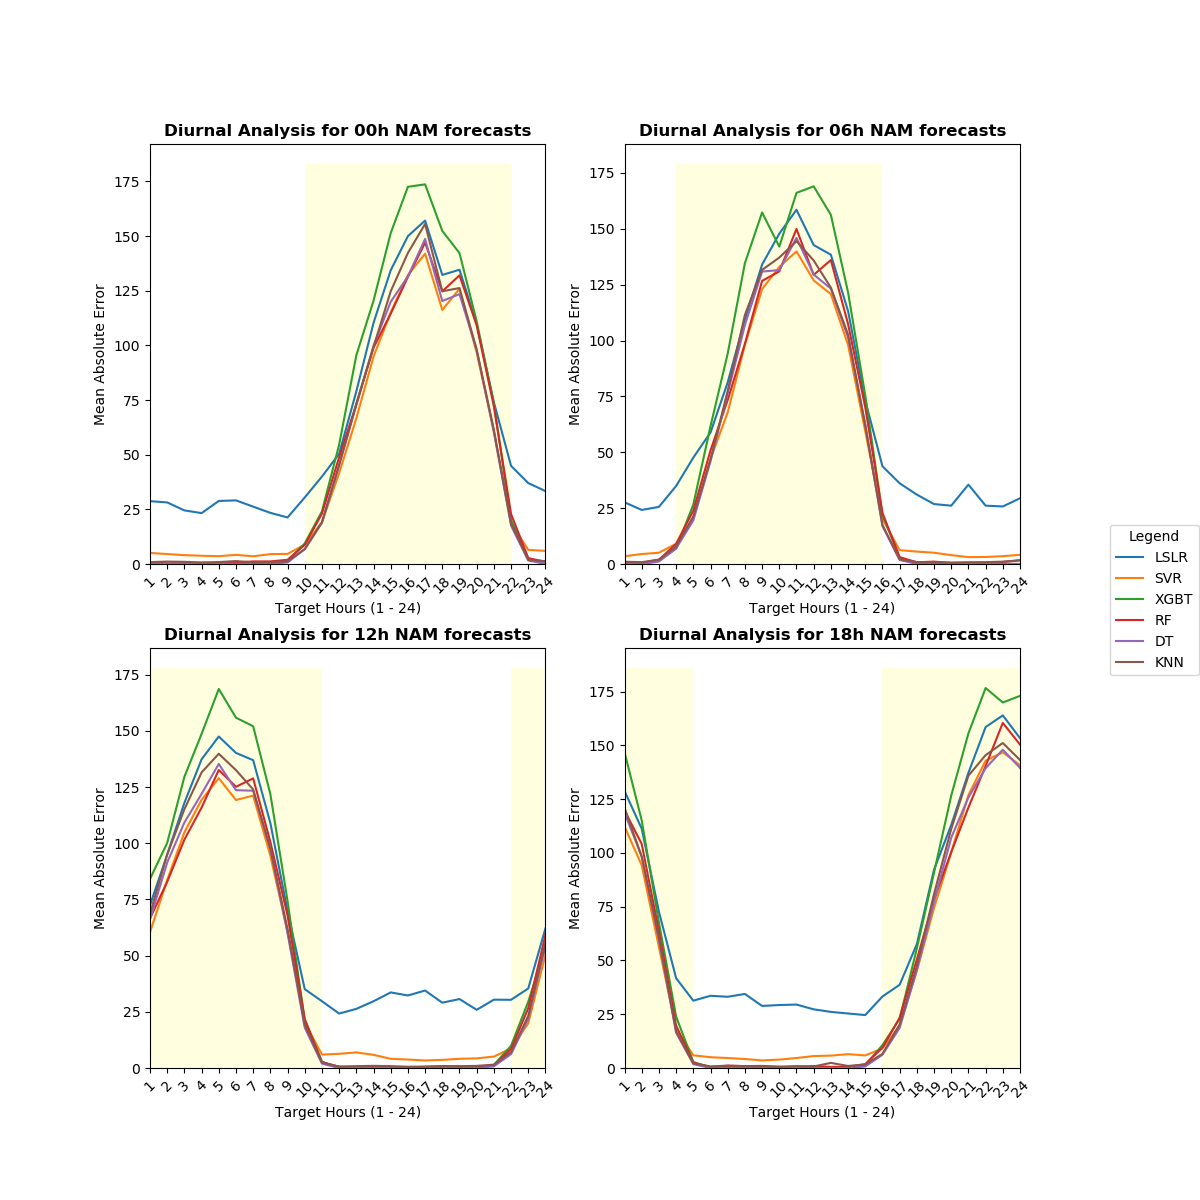
\includegraphics[width=0.9\textwidth, height=12cm]{chapter3/fig_diurnal_arrayb.png}
    	\caption[Stratified diurnal analysis of day-ahead irradiance predictions for fixed-axis solar array]{Stratified diurnal analysis of day-ahead irradiance predictions for fixed-axis array: (left-top) 00h NAM forecasts, (right-top) 16h NAM forecasts, (left-bottom) 12h NAM forecasts, (right-bottom) 18h NAM forecasts. Local time of day (6A.M to 6P.M) at the target location for each of the NAM forecasts is indicated in light yellow.}
    	\label{fig:fig_stratified_diurnal}
    \end{center}
\end{figure}

\par NAM forecasts are released at 00h, 06h, 12h and 18h UTC. In order to assess the performance of the machine learning models as a result of incorporating the input-selection scheme better, a stratified analysis was carried out. The mean absolute error (MAE) of the models for each of the target hours in the forecast horizon, i.e. between 1 and 24 was compared for all four types of NAM forecasts individually.

\par For using weather data from NAM Forecast System for training with the machine learning models, the reference times of the NAM forecasts were made time-zone aware with respect to the target location, i.e. Athens, Georgia. For the reference times corresponding to each of the NAM forecasts, corresponding solar irradiance observations were collected. The target location is -5.00 hours with respect to UTC in the standard time zone, and -4.00 hours with respect to UTC during \textit{daylight saving time}. For the sake of a diurnal analysis, it was assumed that the target location is -4.00 hours with respect to UTC throughout the year. 

\par Thus, 00h, 06h, 12h, 18h NAM forecasts each correspond to 8 P.M, 2 A.M, 8 A.M and 2 P.M locally. In Figure~\ref{fig:fig_stratified_diurnal}, for each of the NAM forecasts, local \textit{time of day} (i.e. between 6.00 AM and 6.00 PM) was identified. In the forecast horizon, i.e. in the consequent 24 hours, for each of the NAM forecasts, such \textit{time of day} was marked in yellow, so as to signify daytime. In Figure~\ref{fig:fig_stratified_diurnal}, it can be seen that the performance of most of the machine learning models is comparable regardless of day-time or night-time. While the \textit{support vector regression} models performed well during daytime, they performed slightly worse during night-time, only performing better than the simple \textit{linear regression}. The stratified diurnal analysis was essential in realizing that the performance of the models in Tables~\ref{Tab:fs_array_a}, \ref{Tab:fs_array_b} and \ref{Tab:fs_array_e} is misleading, as a much higher $MAE$ can be observed for certain target hours in the \textit{time of day}, for each of the forecasts.

\begin{figure}[ht]
    \begin{center}
    \subfloat[Local time analysis of NAM forecasts]{
    	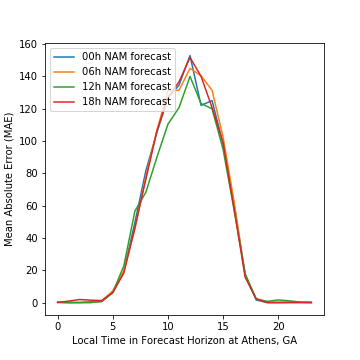
\includegraphics[width=0.5\textwidth, height=8cm]{chapter3/fig_time_shift_analysis.png}        }
%    \hspace{5mm}
    \subfloat[Model comparison at noon (local time)]{
    	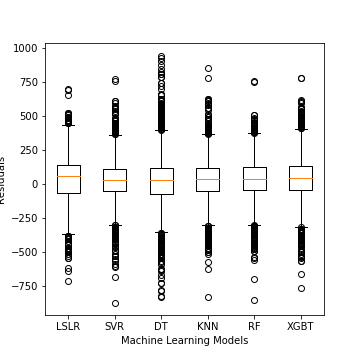
\includegraphics[width=0.5\textwidth, height=8cm]{chapter3/fig_noon_whisker.png}
        }
	\caption[Model performance comparison at different times in a day at the target location.]{ (a) Average performance of different target hours in the forecast horizon corresponding to each of 00h, 06h, 12h, 18h NAM forecasts, adjusted according to local time. 
	(b) Comparison of box-and-whisker plots of residuals from different predictive models utilizing GHI at 12 P.M local time, i.e. noon.}
	\label{fig:local_time_analysis}
    \end{center}
\end{figure}

\par In order to get a better understanding of the performance of the models, a local-time analysis was done. For each of the NAM forecasts, the forecast horizon corresponds to the following time ranges with respect to the target location: 9 P.M - 8 P.M, 3 A.M - 2 A.M, 9 A.M - 8 P.M, 3 P.M - 2 P.M. From these local time ranges, the predictions obtained from the \textit{random forests} algorithm corresponding to target hours representing the same local time were sampled together. $MAE$ was estimated for each of these groups, so as to attain the model performance at a certain time in a day, at the target location. In Fig.~\ref{fig:local_time_analysis}(a), this was plotted for each of the 00h, 06h, 12h, 18h NAM forecasts. The worst performance, expectedly, was observed at 12.00 P.M (local time) or noon. Such an analysis helps realize that for day-ahead solar forecasting with quality weather forecast data, the local time for which the prediction is being made is key to the quality of the prediction, than how farther away the target hour is in the forecast horizon.

\par In order to ascertain the better machine learning model at the local time most difficult to predict solar irradiance for, the quality of prediction of all machine learning models at 12 P.M (local time) was compared. To enable this, in Fig.~\ref{fig:local_time_analysis}(b), box-and-whisker plots were drawn for the residuals of the predictions from all the models at this time. It was observed that the \textit{random forests} had the least dispersion beyond the whiskers, indicating its effectiveness in irradiance prediction irrespective of the position of the target hour in the forecast horizon, or the local time of the target hour.

\newpage
\chapter{}{{Multi-Model Approaches to Solar Forecasting}}{Multi-Model Blending Approaches to Solar Irradiance Forecasting}

\subchapter{Overview}
\par There is a significant variability in the \textit{global horizontal irradiance} (GHI) measured by NWP models with respect to cloud conditions. Mathiesan and Kliessl \cite{multimodel_overpredict} found that the NAM Forecast System tends to overpredict GHI in clear-sky conditions, i.e. sky conditions in which visible clouds are absent, by up to 40 percent. They proposed a bias-correction scheme to selectively correct the overpredicted GHI. In this scheme, they derived a multivariate fourth-order model-output statistics (MOS) correction function depending on solar zenith angle ($\theta_z$) and clear-sky index ($K_c$). Based on $K_c$, sky-conditions for the forecasts were determined. The bias correction function was employed on the forecasts possessing a positive bias in clear-sky conditions. 

\par However, Diagne et al. \cite{litrev_nwp5} noted that this bias-correction methodology was not adequate, as even the accurate forecasts were unnecessarily corrected. Thus, a need for a superior bias-correction methodology depending on cloud-conditions was identified, so as to improve the GHI predicted by the NAM Forecast System. The experiments conducted in this chapter are devoted towards exploring theory-driven approaches for this purpose.

\par There are multiple empirical solar radiation formulations which have been extensively discussed in literature \cite{litrev_pvlib10}\cite{litrev_pvlib11}\cite{litrev_pvlib12}\cite{litrev_pvlib13}\cite{litrev_pvlib14}\cite{litrev_pvlib9}, which compute the different components of solar irradiance from environmental conditions, through experimental observations. These can be broadly classified into \textit{decomposition} and \textit{parametric} models \cite{litrev_pvlib3}. Using assumptions on solar geometry and transmittance, the former are used to estimate direct beam and diffuse irradiance. The latter are useful for approximating daily solar radiation reaching tilted surfaces. In this chapter, two such empirical solar radiation models, \textit{Clear-Sky Scaling} and \textit{Liu-Jordan Model} are discussed, which help estimate different components of global solar radiation, including GHI.

\restoregeometry\noindent
\par In climatic research, in order to be able to distinguish between clear-sky and cloudy-sky conditions effectively, measures such as \textit{clear-sky index} ($K_c$) and \textit{clearness index} ($K_t$) have been introduced. Clear-sky index is generally described as the ratio of measured global horizontal irradiance in a system to its measure in clear-sky conditions, estimated with the help of a clear-sky solar radiation model. It makes accurate and continuous determination of cloud amount from surface measurements possible \cite{multimodel_clearskyindex}. In contrast, clearness index is simply a ratio of the measured irradiance at a location, to the extraterrestrial irradiance calculated at the location. It is extremely useful as it incorporates both light scattering and light absorption, which is beneficial towards estimating the shortwave radiation reaching the surface of the earth.

\par In this work, a theory-driven multi-model blending approach is explored towards correcting the reported bias in GHI. This is done by combining the NAM Forecast System with the empirical \textit{Clear-Sky Scaling} technique based on $K_c$ estimates, and with the \textit{Liu-Jordan} model based on $K_t$ estimates. In the case of the former, the clear-sky Ineichen Model was used to compute the clear-sky GHI, which goes into estimating $K_c$. From among the 00h, 06h, 12h, 18h UTC forecasts released by the NAM Forecast System, 18h NAM forecasts with $K_c > 0.85$ were corrected, by substituting the GHI from NAM Forecast System ($GHI\textsubscript{NAM}$) with the arithmetic mean of the $GHI\textsubscript{NAM}$ and GHI estimates from \textit{Clear-Sky Scaling} technique ($GHI\textsubscript{CS}$). 

\par Predictive models implementing the random forest technique were developed utilizing $GHI\textsubscript{NAM}$ and $GHI\textsubscript{CS}$ independently. The models were compared, and it was observed that such a bias-correction scheme led to an improvement in performance, reducing the mean absolute error ($MAE$) by 4.95\%, 4.53\% and 4.12\% for the dual-axis tracking, fixed-axis and single-axis tracking solar arrays respectively. A similar comparison was performed by including other weather variables from NAM Forecast System, and incorporating the input-selection scheme described in 3.2. However, in this case, the model-blending approach did not lead to an improvement in performance, resulting in an $MAE$ of 72.57 $W/m^2$, 44.91 $W/m^2$ and 63.6 $W/m^2$ for each of the solar arrays.

\par A similar model-blending approach was evaluated for combining the NAM Forecast System with \textit{Liu-Jordan} model, depending on $K_t$ estimates. $K_t$ was computed based on estimations for \textit{extraterrestrial radiation} and \textit{solar zenith angle} for the target location, i.e. Athens, Georgia. For the 18h NAM forecasts with $K_t > 0.35$, $GHI\textsubscript{NAM}$ was substituted with the arithmetic mean of $GHI\textsubscript{NAM}$ and GHI from \textit{Liu-Jordan} model ($GHI\textsubscript{LJ}$). Predictive models implementing the random forests technique were developed, utilizing $GHI\textsubscript{NAM}$ and $GHI\textsubscript{LJ}$ independently as well. It was observed that the former performed better, with the $MAE$ improving by 4.17\%, 4.14\% and 3.62\% for dual-axis tracking, fixed-axis and single-axis tracking solar arrays respectively. Additionally, predictive models implementing random forests technique were developed by including other weather variables from NAM Forecast System, and incorporating the input-selection scheme. For these models, the model-blending technique \textit{slightly deteriorated} the performance, resulting in an $MAE$ of 72.74 $W/m^2$, 45.25 $W/m^2$ and 63.97 $W/m^2$ for each of the solar arrays.

\par In order to study the utility of clear-sky index, another model-blending methodology was explored in which clear-sky index was included as a predictor variable to various machine learning models rather than GHI. The intuition behind this approach was to capture the diurnal and seasonal cyclicity capturing ability of this measure \cite{multimodel_clearskyindex2}. Such an ability can be attributed to the \textit{solar zenith angle}, which goes into the computation of this measure and helps track the position of the Sun. An input-selection scheme in line with that followed in Chapter 3 was used to generate a weather forecast data for the machine learning models, so as to forecast solar irradiance for the dual-axis tracking, fixed-axis and single-axis tracking solar arrays.

\par The performance of such predictive models was worse than that obtained by utilizing the input-selected weather forecast data from the NAM Forecast System (reported in Tables~\ref{Tab:fs_array_a}, \ref{Tab:fs_array_b}, \ref{Tab:fs_array_e}). The $MAE$ increased for the best performing \textit{random forests} by 11.59\%, 9.8\% and 9.42\% along each of the solar arrays, recording an $MAE$ of 79.58 $W/m^2$, 49.18 $W/m^2$ and 69.98 $W/m^2$ respectively. A stratified diurnal and seasonal analysis was performed on the predictions attained through this methodology. The presumed cyclicity-capturing ability of the clear-sky index measure did not translate into improving the performance of the predictive models across corresponding seasons.

\subchapter{Empirical Solar Radiation Models}
\par Solar researchers have developed various formulations through experimental observations, which help in determining the relation between different components of solar radiation and various meteorological parameters. Of these, \textit{parametric} models require information about atmospheric conditions such as turbidity, cloud cover, etc. to be able to formulate the different components of solar irradiance such as diffuse horizontal irradiance (DHI), direct normal irradiance (DNI) and global horizontal irradiance (GHI). \textit{Decomposition} models formulate equations to estimate the solar irradiance components based on the correlations between them. Such formulations are relevant, especially in cases where meteorological data is not adequately available.

\par DHI is the amount of solar radiation received by a horizontal surface, which has been scattered by the molecules and particles in the atmosphere. It is the part of solar radiation which does not belong to the $5^{\circ}$ field of view concentric around the sun. DNI is the direct radiation received on a plane normal to the sun over the total solar spectrum. It is an essential component of global irradiance, especially in cloudless conditions. GHI is the total amount of such terrestrial irradiance which is received by a surface horizontal to the surface of the earth. It can measured with the help of pyranometers, and in general, can be computed from DHI and DNI using the following equation, where $\theta_z$ is the \textit{solar zenith angle} (the angle between sun and the vertical):
\begin{equation}\label{eq:ghi}
    GHI = DHI + DNI . cos(\theta_z)
\end{equation}

\par Holmgrem et al \cite{pvlib_Holmgren2018} contributed to building \textit{pvlib-python}\footnote{\url{https://github.com/pvlib/pvlib-python}} an open source, python-based software, ported from the PVLIB MATLAB toolbox developed at Sandia National Laboratories. This software provides a set of utilities for simulating the performance of the photovoltaic energy systems, with implementations of algorithms related to solar energy. Specifically, it contains components to obtain weather forecast data from NOAA/NCEP/NWS models including the GFS, NAM, RAP, HRRR, and the NDFD, retrieved from the UNIDATA THREDDS servers; and components to convert this weather forecast data into a PV power forecast.

\par For our experiments, we retrieved a NAM data product ($NAM\textsubscript{awphys}$) from the NCEP servers. This is different from the one retrieved by \textit{pvlib-python} ($NAM\textsubscript{awip}$) in that the former is a full complement of both the pressure level fields and surface-based fields, while the latter is a full complement of just the surface-based fields. To be able to extend the solar energy related algorithms to the NAM weather forecast data collected by us, making it compatible with $NAM\textsubscript{awip}$ becomes essential.

\par $NAM\textsubscript{awip}$ data retrieved by \textit{pvlib-python} consists of the following surface-level parameters: air temperature, wind speed, total clouds, low clouds, mid clouds and high clouds. In order to enable the use of \textit{pvlib-python} functionalities on the weather forecast dataset collected by us, equivalent surface-level fields were identified in $NAM\textsubscript{awphys}$. In this work, each of the irradiance metrics GHI, DHI and DNI were computed from the \textit{pvlib-python} compatible NAM dataset using two empirical solar radiation models implemented in the software: Clear-sky Scaling, Liu-Jordan Model.
\vspace{0.3cm}

\subsubchapter{Clear-sky Scaling}
\par Global horizontal irradiance can be measured with the help of a pyranometer on a horizontal surface. For this reason, it is typically the most common type of irradiance measurement. Knowledge of clear sky conditions, i.e. where the visible clouds are absent, is a key requirement for forecasting terrestrial solar radiation. Empirical solar radiation models such as clear-sky models estimate the solar radiation under a cloudless sky based on various atmospheric parameters. Such models can generally be validated by comparing the estimated irradiance with the measured irradiance in clear-sky conditions. 

\par Several parametric models have been proposed in literature to compute the different components of solar radiation from environmental conditions such as atmospheric turbidity, fractional sunshine, perceptible water vapor, etc. Ineichen et al \cite{pvlib_ineichen} formulated a model to compute Linke turbidity independent of the airmass, and clear-sky GHI from this metric. In this technique, the \textit{Ineichen Clear-Sky Model} was used to compute the clear-sky GHI ($GHI\textsubscript{CS}$). Going by Larson et al's \cite{pvlib_larson} work, this was scaled on the basis of the total cloud cover ($TCC$) according to the following equation: 
\begin{equation}\label{eq:ghi_cs}
    GHI = GHI_{CS} . [0.35 + 0.65(1 - TCC)]
\end{equation}

\par In addition, the popular \textit{Direct Insolation Simulation Code} (DISC) model introduced by Maxwell et al. \cite{pvlib_disc} was used to compute the direct beam component of global solar radiation, i.e. DNI. The diffuse part of global solar radiation, i.e. DHI was computed by subjecting the GHI (estimated with Eq.~\ref{eq:ghi_cs}) and DHI to Eq.~\ref{eq:ghi}

%\par Maxwell et al \cite{pvlib_disc} introduced the popular \textit{Direct Insolation Simulation Code} (DISC) model to compute cloudy-sky DNI from GHI (in this case, computed with Eq. \ref{eq:ghi_cs}) and other environmental factors. Clearness index is the fraction of the solar radiation transmitted through the atmosphere to strike the earth's surface. DISC model uses empirical relationships between the direct and global components of this measure to estimate the direct beam component. Additionally, the clear-sky DHI component can be evaluated from these irradiance metrics and the solar zenith angle using the equation described in Eq. \ref{eq:ghi}.

\subsubchapter{Liu-Jordan Model}
\par Decomposition models typically utilize only data pertaining to global solar radiation, to estimate the diffused component. They depend on the atmospheric effects in an isolated place, varying according to time of the year, season and climatic conditions \cite{pvlib_liujordan}. Liu et al. proposed one of the simplest and earliest models of radiation, the Liu-Jordan model \cite{pvlib_liujordan2}, which presumes that diffuse radiation intensity is distributed uniformly over the whole sky. In this model, the diffuse irradiance on a surface tilted towards the equator at an angle $\theta$, where $I_D$ is the diffuse radiation on a horizontal surface is given by the following empirical equation:

\begin{equation}\label{eq:lj_dhi}
    I_{Dt} = I_D . (\frac{1 + cos\theta}{2})
\end{equation}

Liu-Jordan model, though simple, is one of the more accurate models for estimating diffuse radiation on inclined surfaces \cite{pvlib_liujordan3}. This model helps determine DNI, GHI from properties such as extraterrestrial flux, transmittance, and optical air mass number. It has been observed that the Liu-Jordan model provides a good fit to empirical data under overcast skies, but underestimates the solar radiation on tilted surfaces when used for partially-clear and clear-sky days \cite{pvlib_liujordan4}.

\subchapter{Experiment Setup}
\par In this chapter, two series of experiments are performed towards predicting solar irradiance on each of the dual-axis tracking, fixed-axis and single-axis tracking solar arrays. They can be summarized as follows:
\setlist{nolistsep}
\begin{itemize}[noitemsep]
    \item contrasting the utilization of GHI (from NAM Forecast System), adjusted GHI (from blending NAM Forecast System with \textit{Clear-Sky Scaling} and \textit{Liu-Jordan} techniques) as a predictor variable
    \begin{enumerate}[label=(\alph*)]
        \item comparing performance of \textit{random forests} utilizing GHI and adjusted GHI independently as predictors
        \item comparing performance of \textit{random forests} utilizing other input-selected NAM weather variables along with GHI and adjusted GHI as predictors
    \end{enumerate}
    \item contrasting performance of predictive models utilizing \textit{clear-sky index} rather than GHI
\end{itemize}


\par In the first series of experiments, a theory-driven bias-correction scheme combining the NAM Forecast System with empirical solar radiation models such as \textit{Clear-Sky Scaling} and \textit{Liu-Jordan} is explored. In Chapter 3, it was observed that the \textit{random forest} was the best performing machine learning model for the purpose of solar irradiance forecasting. Independent predictive models were developed using this algorithm, utilizing GHI estimates from NAM Forecast System and bias-corrected GHI estimates from model-blending as input. These models were compared and analyzed, so as to gauge the effect of the model-blending scheme. In order to enable a consistent comparison of model performance, evaluation metrics used in Chapter 3, i.e. mean absolute error ($MAE$) and coefficient of determination ($R^2$) were used in this chapter as well. 

\begin{figure}[ht]
    \begin{center}
    	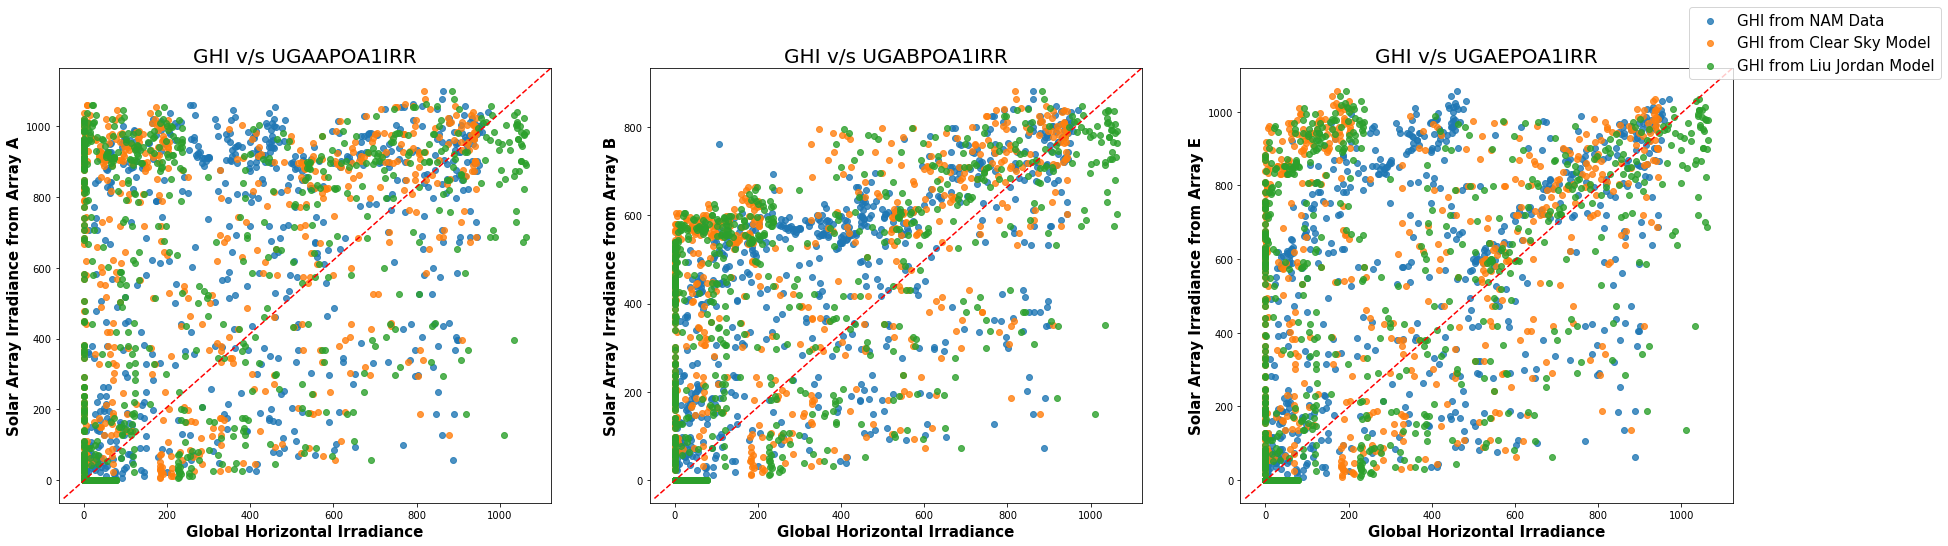
\includegraphics[width=\textwidth]{chapter4/fig_ghi_irradiance.png}
    	\caption[GHI from NAM data, Clear-sky Scaling and Liu-Jordan against irradiance observations from dual-axis tracking, fixed-axis, single-axis tracking solar arrays through 2017.]{Correlation of the first feature projection corresponding to GHI from NAM data, Clear-sky Scaling and Liu-Jordan Model, with respect to irradiance observations from dual-axis tracking (left), fixed-axis (center) and single-axis tracking (right) solar arrays through 2017.}
    	\label{fig:fig_ghi_irradiance}
    \end{center}
\end{figure}

\par Furthermore, other NAM weather variables such as air temperature, height at planetary boundary layer, and total cloud cover, which were observed to be effective for solar irradiance prediction were also considered. 
Predictive models were developed by including these weather variables along with the different variants of GHI described earlier. This weather forecast dataset was input to \textit{random forests} with the input-selection scheme described in 3.2, so as to predict solar irradiance on each of the solar arrays. The performance of these predictive models was compared with models utilizing input-selected NAM weather forecast data, in which the GHI estimates weren't adjusted. 

\par A second series of experiments was performed, where multiple machine learning models were developed using \textit{clear-sky index} rather than GHI, along with the other NAM weather variables. An input-select scheme in line with that in 3.2 was designed to selectively pick relevant feature projections of the weather variables in the forecast horizon. Solar irradiance predictions were made utilizing this weather forecast data on each of the dual-axis tracking, fixed-axis and single-axis tracking solar arrays. A stratified diurnal and seasonal analysis of the performance of these predictive models was performed, to gauge the cyclicity-capturing ability of these models.

\subsubchapter{Blending NAM Forecast System with Empirical Models}
\par \textit{Clear-Sky Scaling} and \textit{Liu-Jordan} techniques were used to evaluate GHI ($GHI\textsubscript{CS}$ and $GHI\textsubscript{LJ}$ respectively) from the meteorological variables in the NAM Forecast System. Both of these GHI estimates were compared with the GHI from the NAM Forecast System ($GHI\textsubscript{NAM}$) for each of the 00h, 06h, 12h and 18h NAM forecasts. In Fig.~\ref{fig:fig_ghi_comparison}, the residuals of the first feature projection of $GHI\textsubscript{CS}$ and $GHI\textsubscript{NAM}$ (left), $GHI\textsubscript{LJ}$ and $GHI\textsubscript{NAM}$ (right) with respect to the corresponding irradiance observations from the fixed-axis solar array were plotted for all NAM forecasts in 2017. 

\par Residuals correspond to the difference between the target irradiance observations and the modeled GHI estimates. Thus, in Fig.~\ref{fig:fig_ghi_comparison}, lying above the X-axis signifies the under-estimation of the corresponding GHI values, and lying under the X-axis signifies the over-estimation of corresponding GHI values. For both the 00h and 06h NAM forecasts, the residuals in both the sub-plots are mostly close to the X-axis, except for a small period for the 00h NAM forecasts. The 00h NAM forecasts correspond to late-evening at the target location. The period for which the residuals corresponding to $GHI\textsubscript{CS}$ and $GHI\textsubscript{LJ}$ are under the X-axis signifies the middle of the year where days are longer, thus leading to possible over-estimation of GHI by the empirical techniques. Meanwhile, the 06h NAM forecasts correspond to night-time at the target location, where there is no sun. Thus, the near-zero residual values for these forecasts are justified. 

\par The residuals of GHI estimates from 12h NAM forecasts are consistently above the X-axis, with those corresponding to the GHI estimates from \textit{Clear-Sky Scaling} and \textit{Liu-Jordan} techniques being constantly greater than the residuals corresponding to the GHI estimates from the NAM Forecast System. This illustrates the under-prediction of GHI by all the modeling techniques, with that from the empirical techniques being greater than the NAM Forecast System. Similarly, residuals corresponding to 18h NAM forecasts are studied as well. However in this case, more variability of the GHI estimates was observed, with a considerable number of over-predicted GHI estimates across all the modeling techniques. 


\begin{figure}
\begin{center}
    \subfloat[NAM Forecast System + Clear-Sky Scaling]{
        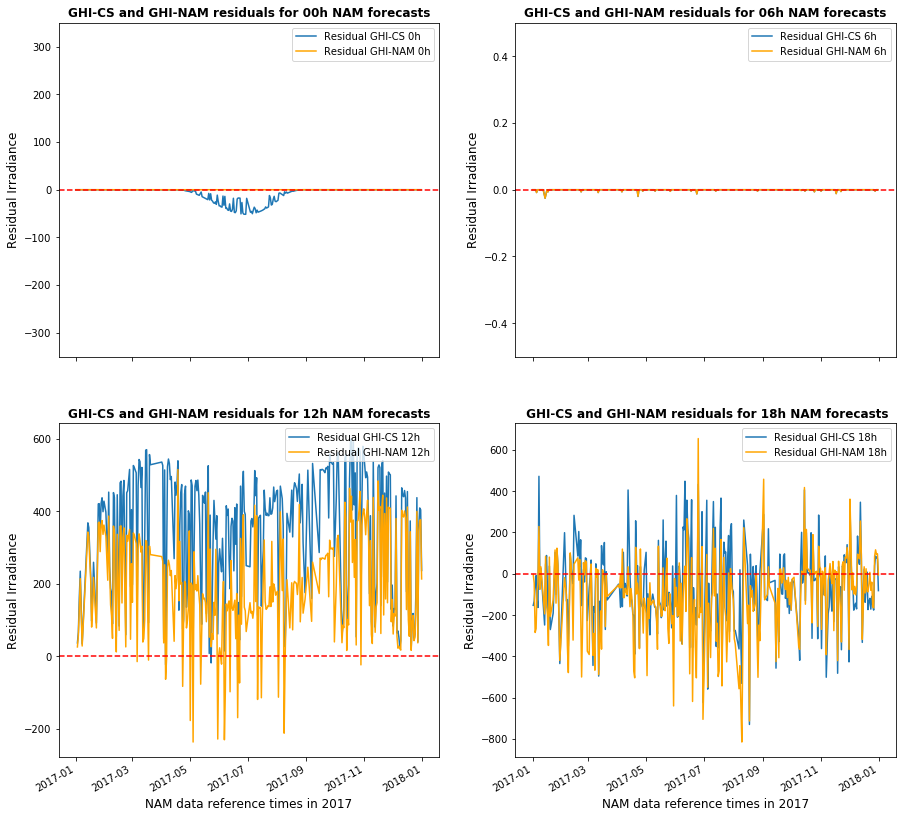
\includegraphics[width=0.46\textwidth]{chapter4/fig_ghi_comparison_cs.png}
        }
    \hspace{5mm}
    \subfloat[NAM Forecast Sytem + Liu Jordan Model]{
        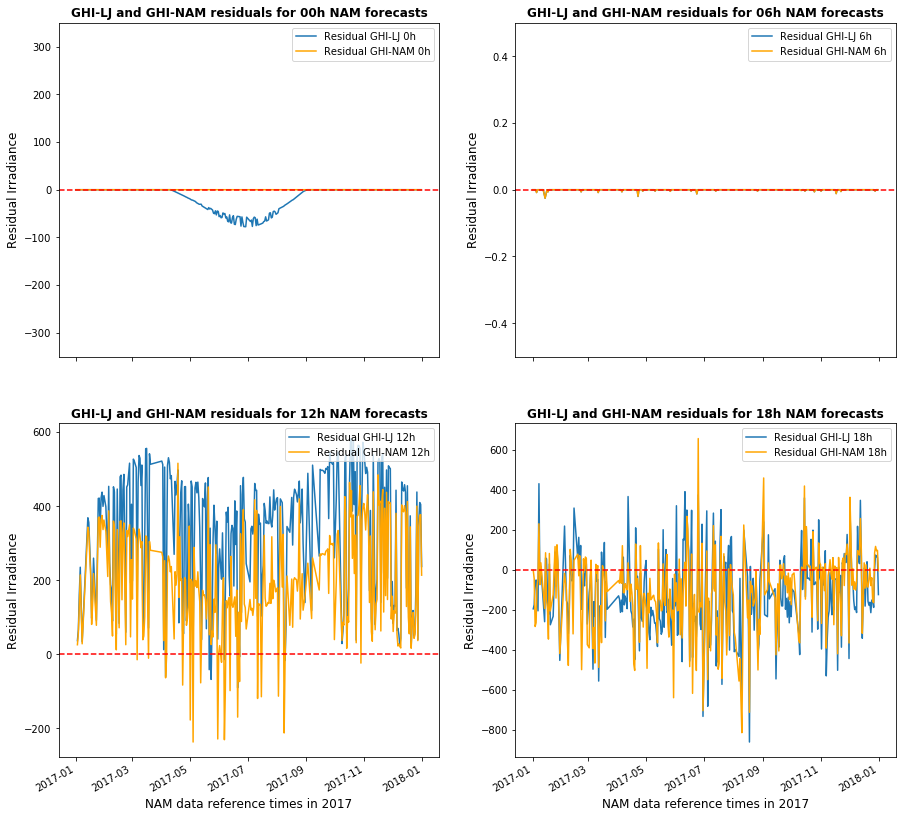
\includegraphics[width=0.46\textwidth]{chapter4/fig_ghi_comparison_lj.png}
        }
    \caption[Comparing GHI estimates from Clearsky-Scaling ($GHI\textsubscript{CS}$) and Liu-Jordan ($GHI\textsubscript{LJ}$ techniques with NAM Forecast System ($GHI\textsubscript{NAM}$ for 00h, 06h, 12h, 18h NAM forecasts]{Comparing GHI estimates from Clearsky-Scaling ($GHI\textsubscript{CS}$) and Liu-Jordan ($GHI\textsubscript{LJ}$ techniques with NAM Forecast System ($GHI\textsubscript{NAM}$ for 00h, 06h, 12h, 18h NAM forecasts: Residuals of $GHI\textsubscript{CS}$ (blue) and $GHI\textsubscript{NAM}$ (orange) with respect to fixed-axis solar array irradiance observations for individual weather forecasts in 2017 (left); Residuals of $GHI\textsubscript{LJ}$ (blue) and $GHI\textsubscript{NAM}$ (orange) with respect to fixed-axis solar array irradiance observations for individual weather forecasts in 2017 (right).}
    \label{fig:fig_ghi_comparison}
\end{center}
\end{figure}

\par To be able to explain the variability in the GHI estimates of the 18h NAM forecasts better, studying measures which determine the amount of cloudiness in the sky is essential. In this regard, \textit{clear-sky index} and \textit{clearness index} were explored. Clear-sky index helps in the removal of diurnal and seasonal signals from a given set of radiation data \cite{expt_clearsky_index}. This can be attributed to the fact that the \textit{solar zenith angle}, i.e. the elevation angle of the Sun is utilized in the estimation of this measure. In contrast, \textit{Clearness index} helps in estimating the clearness in the sky and can be determined for a specific day based on collected meteorological data and knowledge of extraterrestrial irradiance. It is extremely important in the parameterization of \textit{Liu-Jordan} model. 

\par The \textit{Ineichen Model} was used to compute the clear-sky GHI, which goes into the estimation of \textit{clear-sky index}. For the computation of clearness index, estimation of extraterrestrial radiation for a day of the year, and the estimation of solar zenith angle are necessary. Reda et al. \cite{multimodel_spa} proposed \textit{Solar Position Algorithm}, an implementation of which was used in the determination of the solar zenith angle. The extraterrestrial radiation was determined using an implementation of the algorithm described by Spencer. J in \cite{multimodel_extraterrestrial}. Both of these measures were formulated such that the negative and non-finite values are truncated to zero, and the maximum value is 2, allowing the over-irradiance events typically seen in sub-hourly data. In Fig.~\ref{fig:fig_kc_kt_18h}, to further study the variability in $GHI\textsubscript{CS}$ and $GHI\textsubscript{LJ}$, clear-sky index and clearness index were plotted for the 18h NAM forecasts.

\begin{figure}
\begin{center}
    \subfloat[]{
        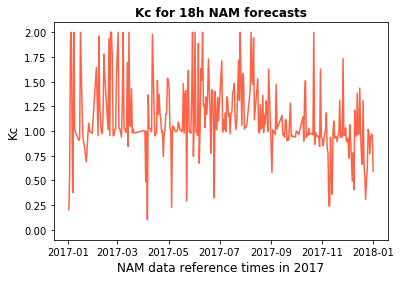
\includegraphics[width=0.46\textwidth]{chapter4/fig_kc_18h.png}
        }
    \hspace{5mm}
    \subfloat[]{
        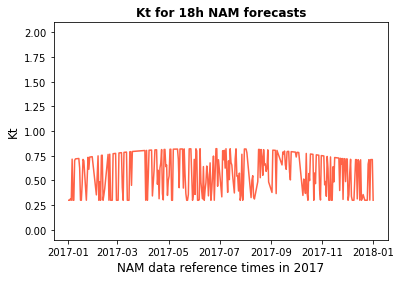
\includegraphics[width=0.46\textwidth]{chapter4/fig_kt_18h.png}
        }
    \caption[Clear-Sky Index and Clearness Index estimates for 18h NAM forecasts in 2017]{Clear-Sky Index ($K_c$, left) estimates and Clearness Index ($K_t$, right) estimates for 18h NAM forecasts in 2017.}
    \label{fig:fig_kc_kt_18h}
\end{center}
\end{figure}

\par Generally, clear-sky index values greater than 1 indicate higher solar irradiance observations. It was observed that the clear-sky index for the 18h NAM forecasts were highly variable, and identifying clear-sky periods based on the clear-sky index was not as straightforward. Thus, a randomized cross-validated grid search was performed to find a threshold for the clear-sky index, above which clear-sky periods could be presumed, and $GHI\textsubscript{NAM}$ could be corrected. The proposed bias-correction involved substituting $GHI\textsubscript{NAM}$ with the arithmetic mean of $GHI\textsubscript{NAM}$ and $GHI\textsubscript{CS}$. Based on such an approach, it was found that $K_c$ could be thresholded at 0.85. For the sake of convenience, in this work, the GHI estimates corresponding to the model-blending techniques will be referred to as \textit{adjusted GHI}, and those corresponding to model-blending between the NAM Forecast System and \textit{Clear-Sky Scaling} as \textit{adjusted} $GHI\textsubscript{NAM+CS}$.

\par A similar randomized cross-validated grid search was performed to identify a threshold for the clearness index as well. For NAM forecasts with clearness index greater than this threshold, sunny conditions could be presumed, and below which, cloudy sky conditions could be presumed. Such a threshold was identified at 0.35. Thus, for all 18h NAM forecasts with $K_t > 0.35$ (i.e. possessing sunny sky conditions), $GHI\textsubscript{NAM}$ was adjusted by substituting it with the arithmetic mean of $GHI\textsubscript{NAM}$ and $GHI\textsubscript{LJ}$. For the sake of convenience, such bias-corrected GHI estimates will be referred to as \textit{adjusted} $GHI\textsubscript{NAM+LJ}$.

\par \textit{Random forests} were the better performing machine learning models for solar irradiance prediction in Chapter 3. Separate predictive models were developed using this algorithm, utilizing $GHI\textsubscript{NAM}$, \textit{adjusted} $GHI\textsubscript{NAM+CS}$ and \textit{adjusted} $GHI\textsubscript{NAM+LJ}$ alone. The performance of each of these models forecasting solar irradiance on the dual-axis tracking, fixed-axis and single-axis tracking solar arrays was compared.

\par In addition, such predictive models were also developed by including additional NAM weather variables along with $GHI\textsubscript{NAM}$, \textit{adjusted} $GHI\textsubscript{NAM+CS}$ and \textit{adjusted} $GHI\textsubscript{NAM+LJ}$ respectively. Relevant feature projections were chosen for each of them based on the input-selection scheme described in 3.2. \textit{Liu-Jordan} model has been shown to be effective in predicting diffuse irradiance on inclined surfaces. This was also verified as the DHI estimated by this technique was highly correlated with ground-based solar irradiance observations. Thus, DHI estimated by \textit{Liu-Jordan} model was included as a predictor to the models involving \textit{adjusted} $GHI\textsubscript{NAM+LJ}$. Performance of models using these three variants of weather forecast data was compared for the dual-axis tracking, fixed-axis and single-axis tracking solar arrays.
\clearpage

\subsubchapter{Predictive Modeling Using Clear-Sky Index}
\par For each of the 25 GHI feature projections in the NAM Forecast System, corresponding clear-sky GHI estimates were computed using the \textit{Ineichen Clear-Sky Model}. These estimates were used to determine the clear-sky index ($K_c$) values, resulting in 25 feature projections for this measure. A higher dependency was observed between $K_c$ and solar irradiance observations from the solar farm, as compared to the other NAM weather variables. Thus, following the input-selection scheme described in 3.2, a mutual information matrix was computed for each of the feature projections of $K_c$ with respect to the solar irradiance observations from fixed-axis solar array in the forecast horizon.

\begin{figure}[htb]
    \begin{center}
    	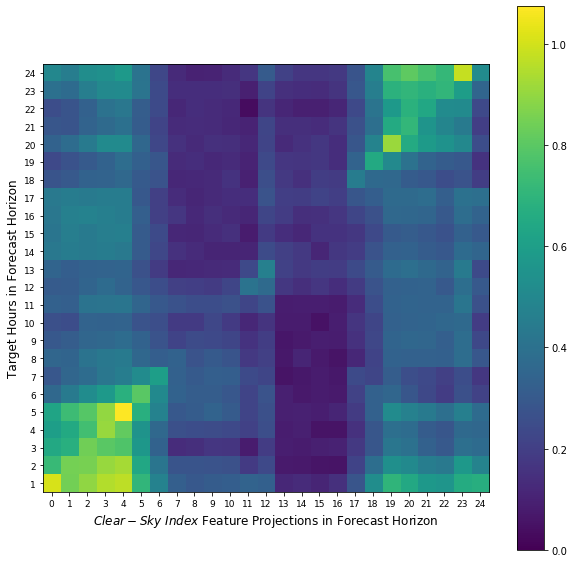
\includegraphics[width=0.65\textwidth]{chapter4/fig_kc_target_mi.png}
    	\caption[Mutual information between Clear-Sky Index feature projections in forecast horizon and irradiance observations for corresponding target hours from fixed-axis solar array]{Mutual information between feature projections of Clear-Sky Index ($K_c$) in the forecast horizon and irradiance observations for corresponding target hours along fixed-axis solar array.}
    	\label{fig:fig_kc_target_mi}
    \end{center}
\end{figure}

\par In Fig.~\ref{fig:fig_kc_target_mi}, it can be seen that the solar irradiance observations are not dependent on all of the $K_c$ feature projections in the forecast horizon. In contrast to the mutual information matrix between the GHI feature projections and solar irradiance observations in the forecast horizon (as in Fig. \ref{fig:fig_ghi_irradiance}), here, the irradiance for a particlar target hour offset in the forecast horizon doesn't necessarily depend on the $K_c$ feature projection corresponding to the same reference time either. As a matter of fact, a lower dependency was observed between the clear-sky index feature projections and target solar irradiance at the center of the forecast horizon.

\par In order to find one such optimal range, a cross-validated grid search was performed. It was identified that the feature projections ranging from 13 hours to 17 hours in the forecast horizon were less relevant. Hence, for the machine learning models trained for each of the target hours, these feature projections were omitted. As a consequence of such an input-selection scheme, 20 feature projections corresponding to clear-sky index and the other NAM weather variables such as air temperature, total cloud cover and height at planetary boundary layer were included as predictors for the machine learning models. Eight temporal encodings (four representing the reference time of the observation, four representing the target hour offset from the reference time) depicting the \textit{time of day} and \textit{time of year} were included as well.

\par Using each of these features as predictors, machine learning models such as \textit{Least-Squares Linear Regression} (LSLR), \textit{k-Nearest Neighbors} (KNN), \textit{Support Vector Regression} (SVR), \textit{Decision Trees} (DT), \textit{Random Forests} (RF) and \textit{Extreme Gradient Boosted Trees} (XGBT) were utilized towards post-processing the solar irradiance from each of the solar arrays. The trivial 24-hour \textit{persistence models} described in Chapter 3 were used as a baseline for this set of experiments as well. For recording the performance of these models, evaluation metrics such as mean absolute error ($MAE$), coefficient of determination ($R^2)$ and Pearson's correlation coefficient ($r$) were used.

\subchapter{Results and Discussion}
\subsubsection*{Assessing Effect of Multi-Model Blending Approaches}
\par In this chapter, the effectiveness of the multi-model blending approaches, i.e. methodologies which combine the NAM Forecast System with the empirical solar radiation models was assessed. Firstly, the performance of the \textit{random forests} algorithm was compared by taking three versions of weather data as input:
\setlist{nolistsep}
\begin{itemize}[noitemsep]
%    \itemsep0em
    \item GHI from NAM Forecast System
    \item adjusted GHI, from blending NAM Forecast System with Clear-Sky Scaling technique \\ (\textit{adjusted} $GHI\textsubscript{NAM+CS}$)
    \item adjusted GHI, from blending NAM Forecast System with Liu-Jordan model \\ (\textit{adjusted} $GHI\textsubscript{NAM+LJ}$)
\end{itemize}

\par In Table \ref{Tab:mmb_array_abe1}, the performance of these predictive models is reported as methodologies \textit{I}, \textit{II} and \textit{III} respectively for each of the dual-axis tracking, fixed-axis and single-axis tracking solar arrays. To enable a smooth comparison with the results reported in chapter 3, and also with the model results from other literature, evaluation metrics such as mean absolute error ($MAE$), coefficient of determination ($R^2$) and Pearson's correlation coefficient ($r$) are reported. The evaluation scheme from Chapter 3, in which the averaged results over 6-hour partitions in the forecast horizon, and the averaged results over the entire forecast horizon is reported, is continued in this chapter too. Both $R^2$ and $r$ over a forecast horizon are computed in a similar fashion as well.
%, by flattening the predictions and ground-truth values for multiple target hours in the forecast horizon into a single array.

\par Random forests utilizing \textit{adjusted} $GHI\textsubscript{NAM+CS}$ performed the best, improving upon those using $GHI\textsubscript{NAM}$ by 4.95\%, 4.53\% and 4.12\% for the dual-axis tracking, fixed axis and single-axis tracking solar arrays respectively. An averaged $MAE$ of 80.61 $W/m^2$, 49.32 $W/m^2$ and 67.52 $W/m^2$ over the entire forecast horizon was reported for each of the solar arrays. An improvement was observed for methodology \textit{III} as well, in which \textit{adjusted} $GHI\textsubscript{NAM+LJ}$ was utilized. Using such a weather forecast dataset resulted in a decrease in $MAE$ by 4.17\%, 4.14\% and 3.62\% respectively, with an $MAE$ of 81.27 $W/m^2$, 49.52 $W/m^2$ and 67.52 $W/m^2$ for the solar arrays.

\vspace{0.6em}

\begin{table}[h]
\begin{center}
    \caption[Evaluating effect of multi-model blending approaches using GHI, on irradiance observations from dual-axis tracking, fixed-axis and single-axis tracking solar arrays, using random forests algorithm.]{Evaluating effect of multi-model blending approaches on irradiance observations from dual-axis tracking, fixed-axis and single-axis tracking solar arrays, using random forests algorithm: \textit{Methodology I} - Using GHI from NAM Forecast System; \textit{Methodology II} - GHI from blending NAM Forecast System and \textit{Clear-Sky Scaling}; \textit{Methodology III} - GHI from blending NAM Forecast System and \textit{Liu-Jordan}.}
    \label{Tab:mmb_array_abe1}
    \begin{tabular}{@{}ccccccccccc@{}}
    \toprule
    \multirow{2}{*}{\textbf{Metric}} & \multirow{2}{*}{\textbf{Horizon}} & \multicolumn{3}{c}{\textbf{Dual-Axis Tracking}} & \multicolumn{3}{c}{\textbf{Fixed-Axis}} & \multicolumn{3}{c}{\textbf{Single-Axis Tracking}}\\
    \cmidrule{3-11}
     &  & \textit{I} & \textit{II} & \textit{III} & \textit{I} & \textit{II} & \textit{III} & \textit{I} & \textit{II} & \textit{III} \\
    
%    \textbf{Metric} & \textbf{Horizon} & \textbf{A} & \textbf{B} & \textbf{C} & \textbf{A} & \textbf{B} & \textbf{C} & \textbf{A} & \textbf{B} & \textbf{C} \\
    \midrule
    \multirow{5}{*}{$MAE$}  & $1 - 6$  & 77.57 & 75.95 & 76.13 & 48.12 & 47.31 & 46.88 & 66.07 & 64.85 & 64.96 \\
           & $6 - 12$       & 86.97 & 83.45 & 83.78 & 52.5  & 51.23 & 51.46 & 72.04 & 69.73 & 69.61 \\
           & $12 - 18$      & 86.62 & 80.43 & 81.05 & 53.13 & 49.42 & 49.89 & 71.04 & 66.1  & 66.79 \\
           & $18 - 24$      & 88.06 & 82.61 & 84.14 & 52.87 & 49.33 & 49.85 & 72.52 & 69.4  & 70.13 \\
           & $Overall$      & 84.81 & \textbf{80.61} & 81.27 & 51.66 & \textbf{49.32} & 49.52 & 70.42 & \textbf{67.52} & 67.87 \\
    \midrule
    \multirow{5}{*}{$R^2$}  & 1 - 6 & 0.86  & 0.86  & 0.86  & 0.91  & 0.91  & 0.91  & 0.87  & 0.87  & 0.87 \\
           & $6 - 12$   & 0.83  & 0.84  & 0.83  & 0.89  & 0.89  & 0.89  & 0.85  & 0.85  & 0.85 \\
           & 12 - 18    & 0.83  & 0.84  & 0.84  & 0.89  & 0.9   & 0.89  & 0.85  & 0.87  & 0.86 \\
           & 18 - 24    & 0.82  & 0.84  & 0.83  & 0.88  & 0.9   & 0.89  & 0.85  & 0.86  & 0.86 \\
           & Overall    & 0.83  & 0.84  & 0.84  & 0.89  & 0.9   & 0.9   & 0.86  & 0.86  & 0.86 \\                     
    \midrule
    \multirow{5}{*}{$r$}  & 1 - 6 & 0.93  & 0.93  & 0.93  & 0.95  & 0.95  & 0.95  & 0.94  & 0.94  & 0.93 \\
           & $6 - 12$   & 0.91  & 0.91  & 0.91  & 0.94  & 0.94  & 0.94  & 0.92  & 0.92  & 0.92 \\
           & 12 - 18    & 0.91  & 0.92  & 0.92  & 0.94  & 0.95  & 0.95  & 0.93  & 0.93  & 0.93 \\
           & 18 - 24    & 0.91  & 0.92  & 0.91  & 0.94  & 0.95  & 0.95  & 0.92  & 0.93  & 0.93 \\
           & Overall    & 0.91  & 0.92  & 0.92  & 0.94  & 0.95  & 0.95  & 0.93  & 0.93  & 0.93 \\                     
    \bottomrule
    \multirow{3}{5em}{Relative Imp. in $MAE$ (\%)} & & & & & & & & & & \\
    & $Overall$ & --- & 4.95\% & 4.17\% & --- & 4.53\% & 4.14\% & --- & 4.12\% & 3.62\% \\ 
    & & & & & & & & & &\\ 
    
    \bottomrule
    \end{tabular}
\end{center}
\end{table}

\par For the next set of experiments, the \textit{random forests} algorithm was combined with the input-selection scheme described in 3.2. This resulted in three versions of input data for the models, in which NAM weather variables such as air temperature, height at planetary boundary layer and total cloud cover were utilized along with the three variants of GHI described earlier. Select feature projections were chosen for each of these meteorological parameters in the predictive models, depending on the target hour offset in the forecast horizon. The results from each of these methodologies is described under \textit{I}, \textit{II} and \textit{III} in Table~\ref{Tab:mmb_array_abe2}.

\par It was observed that both the model-blending approaches observed a slight deterioration in performance. The methodology blending NAM Forecast System with \textit{Clear-Sky Scaling} technique recorded an $MAE$ of 72.57 $W/m^2$, 44.91 $W/m^2$ and 63.56 $W/m^2$ for the dual-axis tracking, fixed-axis and single-axis tracking solar arrays respectively. Meanwhile, combining the NAM Forecast System with Liu-Jordan model recorded an $MAE$ of 72.74 $W/m^2$, 45.25 $W/m^2$ and 63.97 $W/m^2$ for each of the solar arrays.

\begin{table}[h]
\begin{center}
    \caption[Evaluating effect of multi-model blending approaches on irradiance predictions using weather data along dual-axis tracking, fixed-axis and single-axis tracking solar arrays, using random forests algorithm.]{Evaluating effect of multi-model blending approaches on irradiance predictions along dual-axis tracking, fixed-axis and single-axis tracking solar arrays, using random forests algorithm: \textit{Methodology I} - Using input-selected NAM Forecast System; \textit{Methodology II} - Blending input-selected NAM Forecast System and \textit{Clear-Sky Scaling}; \textit{Methodology III} - Blending input-selected NAM Forecast System and \textit{Liu-Jordan}.}
    \label{Tab:mmb_array_abe2}
    \begin{tabular}{@{}ccccccccccc@{}}
    \toprule
    \multirow{2}{*}{\textbf{Metric}} & \multirow{2}{*}{\textbf{Horizon}} & \multicolumn{3}{c}{\textbf{Dual-Axis Tracking}} & \multicolumn{3}{c}{\textbf{Fixed-Axis}} & \multicolumn{3}{c}{\textbf{Single-Axis Tracking}}\\
    \cmidrule{3-11}
     &  & \textit{I} & \textit{II} & \textit{III} & \textit{I} & \textit{II} & \textit{III} & \textit{I} & \textit{II} & \textit{III} \\
    \midrule
     \multirow{5}{*}{$MAE$}  & 1 - 6 & 68.5  & 70.11 & 70.56 & 42.26 & 42.87 & 43.34 & 60.5  & 61.53 & 62.11 \\
           & $6 - 12$   & 72.55 & 72.82 & 73.05 & 45.49 & 45.16 & 45.37 & 63.98 & 63.88 & 64.41 \\
           & 12 - 18    & 70.65 & 72.59 & 72.71 & 44.75 & 45.22 & 45.22 & 62.75 & 63.67 & 63.38 \\
           & 18 - 24    & 74.97 & 74.77 & 74.66 & 46.65 & 46.39 & 47.06 & 66.34 & 65.15 & 65.98 \\
           & Overall    & \textbf{71.67} & 72.57 & 72.74 & \textbf{44.79} & 44.91 & 45.25 & \textbf{63.39} & 63.56 & 63.97 \\                     

    \midrule
    \multirow{5}{*}{$R^2$}  & 1 - 6 & 0.88  & 0.88  & 0.88  & 0.92  & 0.92  & 0.92  & 0.89  & 0.89  & 0.89 \\
           & $6 - 12$   & 0.87  & 0.87  & 0.87  & 0.91  & 0.91  & 0.91  & 0.87  & 0.87  & 0.87 \\
           & 12 - 18    & 0.87  & 0.87  & 0.87  & 0.91  & 0.91  & 0.91  & 0.88  & 0.88  & 0.88 \\
           & 18 - 24    & 0.86  & 0.86  & 0.86  & 0.9   & 0.91  & 0.9   & 0.87  & 0.87  & 0.87 \\
           & Overall    & 0.87  & 0.87  & 0.87  & 0.91  & 0.91  & 0.91  & 0.88  & 0.88  & 0.88 \\                     
    \midrule
    \multirow{5}{*}{$r$}  & 1 - 6 & 0.94  & 0.94  & 0.94  & 0.96  & 0.96  & 0.96  & 0.94  & 0.94  & 0.94 \\
           & $6 - 12$   & 0.93  & 0.93  & 0.93  & 0.95  & 0.96  & 0.95  & 0.93  & 0.93  & 0.93 \\
           & 12 - 18    & 0.93  & 0.93  & 0.93  & 0.95  & 0.96  & 0.96  & 0.94  & 0.94  & 0.94 \\
           & 18 - 24    & 0.93  & 0.93  & 0.93  & 0.95  & 0.95  & 0.95  & 0.93  & 0.93  & 0.93 \\
           & Overall    & 0.93  & 0.93  & 0.93  & 0.95  & 0.96  & 0.96  & 0.94  & 0.94  & 0.94 \\                     

    \bottomrule
    \end{tabular}
\end{center}
\end{table}

\par In general, the addition of weather variables has shown to incorporate site-specific information into the predictive models. In Chapter 3, the selective picking of feature projections of NAM weather variables in the forecast horizon improved the performance of the predictive models considerably. A similar improvement in performance was expected by including additional weather data with the model-blended GHI as well. However, this wasn't the case. This can possibly be attributed to the misidentification of clear-sky conditions by clear-sky index and clearness index respectively. Such a misidentification could have led to an adjustment in GHI, where it wasn't needed.

\subsubsection*{Performance Evaluation for Predictive Modeling using Clear-Sky Index}
\par In this series of experiments, meteorological variables including relevant NAM weather variables and clear-sky index was utilized. The machine learning models were trained on such weather data corresponding to 2017, and evaluated against that corresponding to 2018. For the dual-axis tracking solar array, all the models performed better than the baseline $t-24$ persistence models, which was expected. \textit{Random forests} performed the best, recording an $MAE$ of 79.58 $W/m^2$. However, this was worse in comparison to the performance of this model utilizing input-selected NAM forecast data (as in Table~\ref{Tab:fs_array_a}), for which an $MAE$ of 72.63 $W/m^2$ was observed. In addition, a considerable degradation in performance was observed in the performance of \textit{support vector regression}, the $MAE$ of which increased from 73.43 $W/m^2$ to 83.2 $W/m^2$, and for \textit{k-nearest neighbors}, whose $MAE$ increased from 73.02 $W/m^2$ to 98.52 $W/m^2$.

\begin{table}[h]
\begin{center}
    \caption{Evaluating performance of predictive models using Clear-Sky Index, for irradiance predictions along dual-axis tracking solar array.}
    \vspace{0.2cm}
    \label{Tab:mmb_array_a}
    \begin{tabular}{ccccccccc}
    \toprule
    \textbf{Metric} & \textbf{Horizon} & \textbf{PER} & \textbf{LSLR} & \textbf{SVR} & \textbf{KNN} & \textbf{DT} & \textbf{RF} & \textbf{XGBT} \\
    \midrule
    \multirow{5}{*}{$MAE$}  & $1 - 6$ & 153.32 & 119.41 & 80.21 & 99.59  & 75.96 & 78.52 & 78.52 \\
                            & $7 - 12$ & 153.91 & 134.82 & 82.3  & 94.59  & 79.9  & 77.8  & 79.98 \\
                            & $13 - 18$ & 154.16 & 118.45 & 84.08 & 98.35  & 82.29 & 80.44 & 80.63 \\
                            & $19 - 24$ & 161.43 & 134.98 & 86.19 & 101.54 & 83.76 & 81.55 & 81.36 \\
                            & $Overall$ & 155.71 & 126.92 & 83.2  & 98.52  & 80.48 & \textbf{79.58} & 80.12 \\
                            \midrule
    \multirow{5}{*}{$R^2$}  & $1 - 6$ & 0.46 & 0.82   & 0.87  & 0.71   & 0.86  & 0.86  & 0.86  \\
                            & $7 - 12$ & 0.45 & 0.78   & 0.86  & 0.74   & 0.85  & 0.86  & 0.85  \\
                            & $13 - 18$ & 0.45 & 0.82   & 0.86  & 0.72   & 0.84  & 0.85  & 0.85  \\
                            & $19 - 24$ & 0.41 & 0.76   & 0.84  & 0.71   & 0.84  & 0.85  & 0.85  \\
                            & $Overall$ & 0.44 & 0.79   & 0.85  & 0.72   & 0.85  & 0.85  & 0.85  \\
                            \midrule
    \multirow{5}{*}{$r$}    & $1 - 6$ & 0.73 & 0.91   & 0.93  & 0.86   & 0.93  & 0.93  & 0.93  \\
                            & $7 - 12$ & 0.73 & 0.88   & 0.93  & 0.87   & 0.92  & 0.93  & 0.92  \\
                            & $13 - 18$ & 0.73 & 0.91   & 0.93  & 0.86   & 0.92  & 0.92  & 0.92  \\
                            & $19 - 24$ & 0.71 & 0.87   & 0.92  & 0.85   & 0.91  & 0.92  & 0.92  \\
                            & $Overall$ & 0.72 & 0.89   & 0.93  & 0.86   & 0.92  & 0.93  & 0.92 \\    
    \bottomrule
    \end{tabular}
\end{center}
\end{table}

\par \textit{k-Nearest Neighbors} algorithm does not make any assumptions about the distribution of the data. In this methodology, the feature projections corresponding to GHI are replaced with those of clear-sky index, which have a lesser bias and variance as compared to the former. Thus, a more rigorous cross-validated grid search can be performed to find a better set of hyperparameters. Doing so  might improve the model complexity and help in attaining a better model fit. 

\par The decrease in performance of \textit{support vector regression} can posssibly be attributed to the $C$ hyperparameter, which represents the strength of regularization. With the change in data distribution due to the substitution of GHI feature projections with those corresponding to clear-sky index, the decrease in bias should be compensated with an increase in $C$. Doing so would decrease the regularization penalty on the predictive models, and might improve the performance. This was not accounted for during the training of the predictive models using clear-sky index.

\begin{table}[h]
\begin{center}
    \caption{Evaluating performance of predictive models using Clear-Sky Index, for irradiance predictions along fixed-axis solar array.}
    \vspace{0.2cm}
    \label{Tab:mmb_array_b}
%    \begin{tabular}{@{}p{5.3em}cccccccc@{}}
    \begin{tabular}{ccccccccc}
    \toprule
    \textbf{Metric} & \textbf{Horizon} & \textbf{PER} & \textbf{LSLR} & \textbf{SVR} & \textbf{KNN} & \textbf{DT} & \textbf{RF} & \textbf{XGBT} \\ 
    \midrule
    \multirow{5}{*}{$MAE$} & $1 - 6$ & 111.23 & 76.68 & 50.51 & 59.50  & 48.07 & 48.25 & 50.62 \\
                             & $7 - 12$ & 111.51 & 84.61 & 52.89 & 60.35 & 52.34 & 47.76 & 51.36 \\
                             & $13 - 18$ & 111.97 & 81.33 & 54.87 & 64.85 & 53.68 & 49.55 & 50.92 \\
                             & $19 - 24$ & 117.15 & 88.48 & 56.06 & 63.35 & 53.55 & 51.17 & 51.87 \\
                             & $Overall$ & 112.96 & 82.77 & 53.58 & 62.01 & 51.91 & \textbf{49.18} & 51.20 \\
    \midrule
    \multirow{5}{*}{$R^2$} & $1 - 6$ & 0.59 & 0.88  & 0.91  & 0.83  & 0.90 & 0.91 & 0.90 \\
                             & $7 - 12$ & 0.58 & 0.86  & 0.90   & 0.82  & 0.89  & 0.90 & 0.89 \\
                             & $13 - 18$ & 0.58 & 0.87  & 0.90   & 0.80   & 0.89  & 0.90 & 0.90 \\
                             & $19 - 24$ & 0.55 & 0.83  & 0.88  & 0.81  & 0.88  & 0.90 & 0.89 \\
                             & $Overall$ & 0.58 & 0.86  & 0.90   & 0.81  & 0.89  & 0.90 & 0.90 \\ 
    \midrule
    \multirow{5}{*}{$r$}    & $1 - 6$ & 0.79 & 0.94  & 0.96  & 0.91 & 0.95  & 0.96 & 0.95  \\
                            & $7 - 12$ & 0.79 & 0.93  & 0.95  & 0.91 & 0.95  & 0.95 & 0.95  \\
                            & $13 - 18$ & 0.79 & 0.93  & 0.95  & 0.90 & 0.94  & 0.95 & 0.95  \\
                            & $19 - 24$ & 0.78 & 0.91  & 0.94  & 0.90 & 0.94  & 0.95 & 0.95  \\
                            & $Overall$ & 0.79 & 0.93  & 0.95  & 0.90 & 0.94  & 0.95 & 0.95  \\
    \bottomrule
    \end{tabular}
\end{center}
\end{table}

\par Similar trends were observed for the predictions along fixed-axis and single-axis tracking solar arrays as well. \textit{Random forests} performed the best, recording an $MAE$ of 49.18 $W/m^2$ and 69.98 $W/m^2$ respectively for each of the solar arrays. This performance was worse when compared with the best accuracy obtained by machine learning models utilizing input-selected NAM weather dataset (as in Table~\ref{Tab:fs_array_b} and Table~\ref{Tab:fs_array_e}). There, an $MAE$ of 44.94 $W/m^2$ and 63.60 $W/m^2$ was recorded for both the solar arrays respectively. Though the overall performance of predictive models using clear-sky index worsened, in order to examine the cyclicity-capturing ability of these models, a stratified diurnal and seasonal analysis of the performance of the predictive models with respect to target irradiance predictions on the fixed-axis solar array is performed. 

\begin{table}[h]
\begin{center}
    \caption{Evaluating performance of predictive models using Clear-Sky Index, for irradiance predictions along single-axis tracking solar array.}
    \vspace{0.2cm}
    \label{Tab:mmb_array_e}
    \begin{tabular}{ccccccccc}
    \toprule
    \textbf{Metric} & \textbf{Horizon} & \textbf{PER} & \textbf{LSLR} & \textbf{SVR} & \textbf{KNN} & \textbf{DT} & \textbf{RF} & \textbf{XGBT} \\
    \midrule
    \multirow{5}{*}{$MAE$} & $1 - 6$ & 128.64 & 94.40   & 68.81 & 85.56 & 68.16 & 69.6 & 70.55 \\
                             & $7 - 12$ & 128.97 & 107.51 & 72.16 & 81.62 & 72.58 & 68.46 & 69.09 \\
                             & $13 - 18$ & 129.25 & 98.92  & 72.48 & 87.56 & 72.49 & 69.39 & 69.50 \\
                             & $19 - 24$ & 135.35 & 102.31 & 73.88 & 86.56 & 74.25 & 72.45 & 72.84\\
                             & $Overall$ & 130.55 & 100.78 & 71.83 & 85.33 & 71.87 & \textbf{69.98} & 70.50 \\ 
    \midrule
    \multirow{5}{*}{$R^2$} & $1 - 6$ & 0.53 & 0.85   & 0.87  & 0.75  & 0.86  & 0.87 & 0.86 \\
                             & $7 - 12$ & 0.53 & 0.81   & 0.86  & 0.77  & 0.85  & 0.86 & 0.86 \\
                             & $13 - 18$ & 0.53 & 0.84   & 0.86  & 0.74  & 0.85  & 0.86 & 0.86 \\
                             & $19 - 24$ & 0.49 & 0.83   & 0.86  & 0.75  & 0.85  & 0.86 & 0.86 \\ 
                             & $Overall$ & 0.52 & 0.82   & 0.85  & 0.74  & 0.84  & 0.85 & 0.85 \\
    \midrule
    \multirow{5}{*}{$r$}    & $1 - 6$ & 0.77 & 0.92 & 0.94  & 0.88  & 0.93  & 0.93 & 0.93  \\
                            & $7 - 12$ & 0.77 & 0.90 & 0.93  & 0.89  & 0.92  & 0.93 & 0.92  \\
                            & $13 - 18$ & 0.75 & 0.92 & 0.93  & 0.87  & 0.92  & 0.93 & 0.93  \\
                            & $19 - 24$ & 0.75 & 0.91 & 0.92  & 0.87  & 0.92  & 0.92 & 0.92  \\
                            & $Overall$ & 0.76 & 0.91 & 0.93  & 0.87  & 0.92  & 0.93 & 0.93   \\
    \bottomrule
    \end{tabular}
\end{center}
\end{table}

\subsubsection*{Stratified Diurnal and Seasonal Analysis of Performance}

\par The stratified diurnal analysis conducted in Chapter 3 was extended to the predictive models utilizing clear-sky index as well. In Fig.~\ref{fig:fig_stratified_diurnal_kc}, the performance of the machine learning models for all target hours in the forecast horizon, were plotted for each of the 00h, 06h, 12h and 18h UTC NAM forecasts individually. The time of day was presumed to be between 6 A.M and 6 P.M at the target location, and was highlighted in yellow. In general, as was expected, it was observed that most of the models were able to detect the period of darkness, i.e. night-time relatively well.

\begin{figure}[ht]
    \begin{center}
    	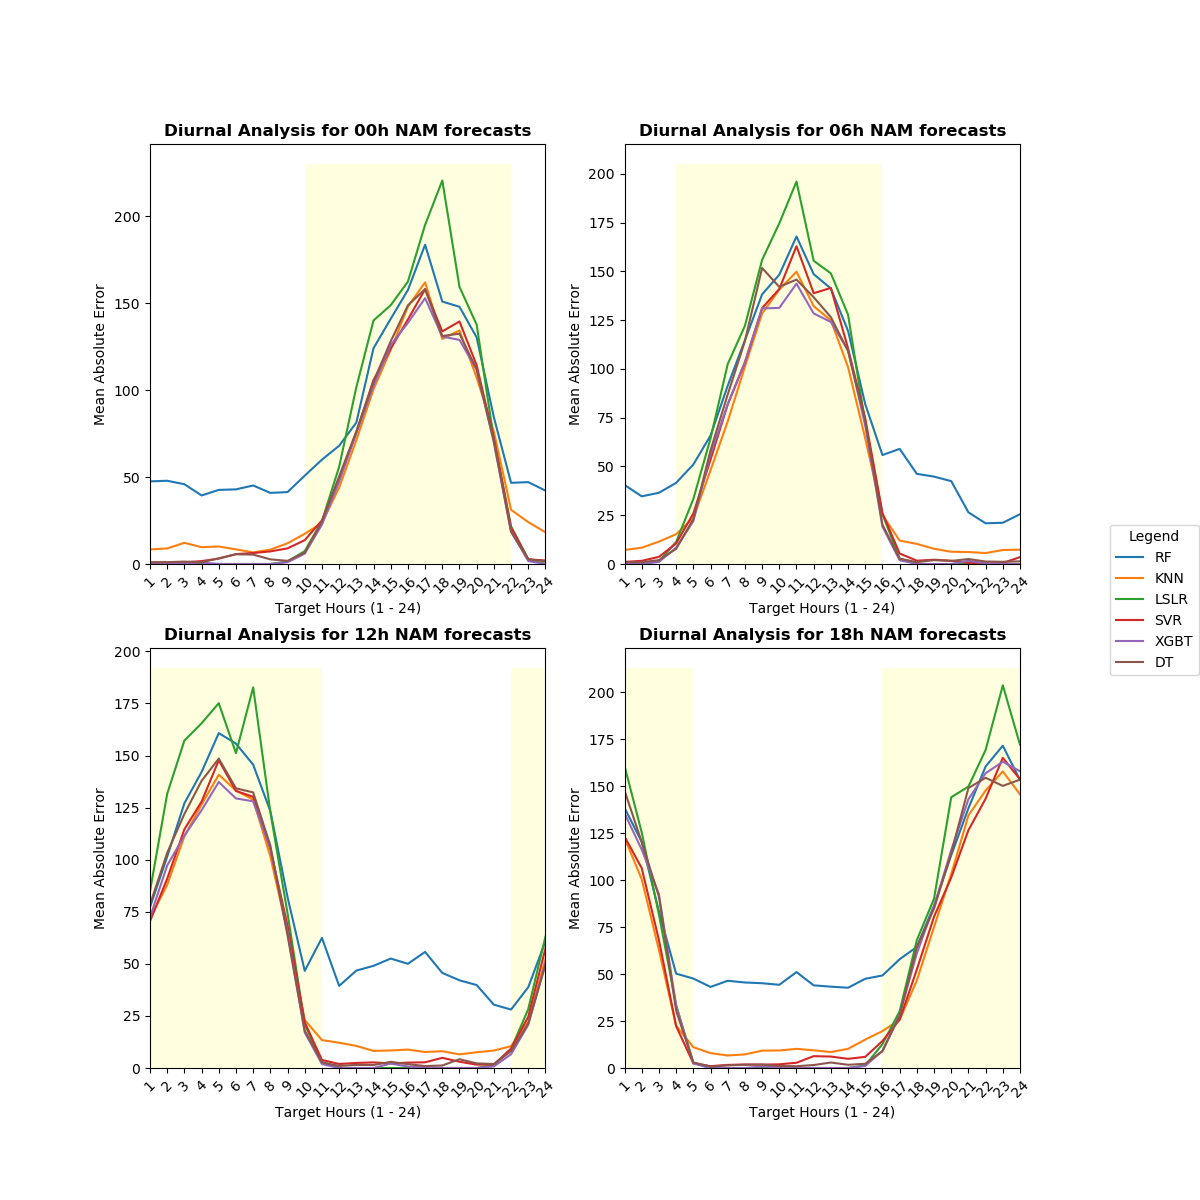
\includegraphics[width=0.9\textwidth, height=12cm]{chapter4/fig_diurnal_arrayb.png}
    	\caption[Stratified diurnal analysis of day-ahead irradiance predictions using Clear-Sky Index for fixed-axis solar array]{Stratified diurnal analysis of day-ahead irradiance predictions using Clear-Sky Index for fixed-axis solar array: (left-top) 00h NAM forecasts, (right-top) 16h NAM forecasts, (left-bottom) 12h NAM forecasts, (right-bottom) 18h NAM forecasts. Local time of day (6A.M to 6P.M) at the target location for each of the NAM forecasts is indicated in light yellow.}
    	\label{fig:fig_stratified_diurnal_kc}
    \end{center}
\end{figure}


\par For the period of day, the more sophisticated machine learning algorithms like \textit{k-nearest neighbors}, \textit{support vector regression} and \textit{random forests} performed better than \textit{decision trees}, and understandably, \textit{linear regression}. However, interestingly enough, \textit{extreme gradient boosted trees} failed to capture day-time well for all the NAM forecasts. This can possibly be attributed to a lesser number of decision trees being used in the ensemble technique. In addition, the diurnal performance of the best performing \textit{random forests} with respect to its performance when utilizing the input-selected NAM weather forecast data (as shown in Fig.~\ref{fig:fig_stratified_diurnal}) can be summarized in the following way:
\setlist{nolistsep}
\begin{itemize}[noitemsep]
    \item performed worse for all the target hours in the day-time for the 00h NAM forecasts
    \item performed better for the target hours 8 through 12 in the forecast horizon, for the 06h NAM forecasts
    \item performed better for the target hours 22 through 24 in the forecast horizon, for the 12h NAM forecasts
    \item performed worse for all the target hours in the day-time for the 18h NAM forecasts
\end{itemize}

\par The target location, i.e. Athens, Georgia is -5.00 hours with respect to UTC in the standard time zone, and -4.00 hours with respect to UTC during \textit{daylight saving time}. To be able to conduct a uniform analysis of the individual NAM forecasts, it was assumed that the local time at the target location is constantly -4.00 hours relative to UTC. 

\par Based on this assumption, as was done in Chapter 3, the performance of different predictive models was compared by analyzing their residuals corresponding to the target hour in the forecast horizon, representing noon, i.e. 12 P.M locally at Athens, Georgia. In Fig.~\ref{fig:fig_noon_whisker}, box-and-whisker plots were drawn corresponding to the residuals from each of the predictive models, so as to study their distributional characteristics. In the figure, the size of the box-plots for most of the models is comparable. In addition, the spread of the residuals beyond the whiskers is minimum for \textit{random forests}, indicating that it is the better machine learning technique for this variant of weather data.

\begin{figure}[ht]
    \begin{center}
%    	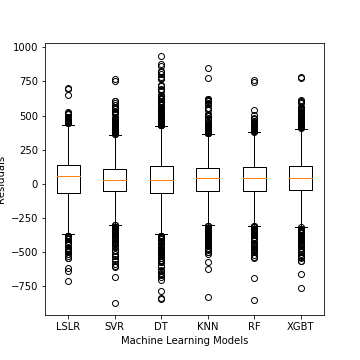
\includegraphics[width=0.75\textwidth, height=8cm]{chapter4/fig_whiskers_csi.png}
    	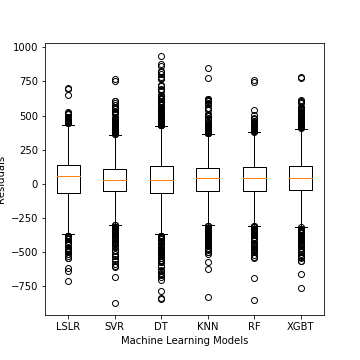
\includegraphics[scale=0.75]{chapter4/fig_whiskers_csi.png}
    	\caption[Comparison of box-and-whisker plots of residuals from different predictive models utilizing clear-sky index at 12 P.M local time]{Comparison of box-and-whisker plots of residuals from different predictive models utilizing clear-sky index at 12 P.M local time, i.e. noon.}
    	\label{fig:fig_noon_whisker}
    \end{center}
\end{figure}

\par Furthermore, a stratified seasonal analysis was conducted for NAM forecasts. It was extended to the 12h and 18h NAM forecasts, which, under the above assumption, represent 8 A.M and 12 P.M locally. Based on the general seasonal trends in the target location i.e. Athens, Georgia, the periods in a year were divided into four seasons: \textit{summer} (May - July), \textit{autumn} (August - October), \textit{winter} (November - January) and \textit{spring} (February - April).

\begin{table}[htbp]
\begin{center}
\caption[Comparing seasonal performance of random forests using input-selected NAM data with GHI and Clear-Sky Index for 12h, 18h NAM forecasts]{Comparing seasonal performance (in $MAE$) of random forests using input-selected NAM data with GHI (left) and clear-sky index (right) for 12h, 18h NAM forecasts.}
\label{tab:seasonal_comparison}
\begin{tabular}{cccccc}
\toprule
\multirow{2}{*}{\textbf{Model}} & \multirow{2}{*}{\textbf{Hour}} & \multicolumn{4}{c}{\textbf{NAM using GHI} / \textbf{NAM using Clear-Sky Index}}   \\ \cmidrule{3-6} 
& & \textit{Summer} & \textit{Autumn} & \textit{Winter} & \textit{Spring} \\
\midrule
LSLR           & 12h                    & 60.21 / 67.41           & 86.35 / 106.9           & 99.71 / 121.9           & 119.4 / 138.1 \\
               & 18h                    & 84.93 / 112.9          & 95.13 / 121.0           & 70.82 / 91.61           & 38.68 / 49.09 \\
SVR            & 12h                    & 46.95 / 64.11          & 64.01 / 74.95           & 72.02 / 88.05           & 84.52 / 102.6   \\
               & 18h                    & 76.11 / 102.4           & 78.75 / 94.32           & 49.03 / 60.49           & 12.39 / 19.49 \\
DT             & 12h                    & 74.60 / 90.51           & 104.4 / 107.9          & 101.8 / 116.4          & 128.3 / 171.6 \\
               & 18h                    & 110.8 / 127.7          & 109.2 / 124.8           & 57.45 / 85.56           & 24.34 / 36.59 \\
KNN            & 12h                    & 54.16 / 58.54          & 81.13 / 83.87           & 89.93 / 90.19           & 98.44 / 87.89 \\
               & 18h                    & 87.39 / 102.5          & 87.52 / 102.4          & 62.32 / 74.12           & 16.25 / 18.76 \\
RF             & 12h                    & 56.15 / 75.93           & 82.91 / 101.9          & 95.77 / 114.0          & 107.5 / 123.0 \\
               & 18h                    & 80.52 / 139.3           & 81.73 / 119.8           & 56.84 / 94.25          & 10.47 / 29.03 \\
XGBT           & 12h                    & 54.07 / 74.41          & 86.37 / 98.35           & 101.1 / 123.3          & 119.2 / 126.0 \\
               & 18h                    & 80.66 / 134.9          & 85.68 / 128.1           & 56.24 / 96.10          & 10.50 / 27.75 \\ \bottomrule
\end{tabular}
\end{center}
\end{table}

\par In Table~\ref{tab:seasonal_comparison}, the performance of the better-performing \textit{random forests} across each of these seasons was compared. The $MAE$ corresponding to predictions of the models utilizing NAM data involving both GHI and clear-sky index was included. It can be observed that the predictive models using clear-sky index performed poorly for both the 12h and 18h NAM forecasts across all the seasons. Moreover, as was noted earlier in the diurnal analysis, the 18h NAM forecasts performed poorly for all the target hours in the forecast horizon. Owing to the relatively poor performance of the NAM forecasts involving clear-sky index, as against those involving GHI, it can be concluded that using the clear-sky index as a predictor in the machine learning models failed to improve the diurnal and seasonal trend capturing ability of the models.



\newpage
\chapter{}{Conclusions and Future Work}{Conclusions and Future Work}

In this thesis, we propose a framework for generalized zero-shot learning (ZSL) that is simple yet very effective. The proposed framework offers an intuitive approach to aid in the training data collection process for image recognition tasks by identifying representative classes using various clustering techniques. It also  provides a method to infer unseen classes using cosine similarity measure. The proposed framework achieves accuracy figures that are 21\% greater on the AWA2 data set and 6\% greater on the CUB data set when compared to the well known Attribute Label Embedding (ALE) scheme for GZSL. On the SUN data set, the proposed model exhibits performance that is comparable to that of ALE. We also determine the minimum number of categories needed to considered as seen classes to achieve reasonable classification accuracy results on all the three data sets using the proposed model.

\par
\medskip

One of the drawbacks of the proposed framework is the inability to infer unseen classes that are distant from the representative classes in the semantic space. There is significant scope for future improvement of the proposed framework in this aspect. A potential solution could be a scheme to map the distance between each unseen class and representative class in a cluster to the classification probabilities obtained from the visual classifier. In this way, the framework would be able to infer all unseen classes, regardless of the distance, with some non-zero probability.

\par
\medskip

Another important future task is the evaluation of the proposed framework on a very large data set such as ImageNet. ImageNet spans more than 1000 classes and has several images in each class unlike the SUN data set which while having over 700 classes, has very few images per class.

\newpage

% Add 'References' section to Table of Contents
\addcontentsline{chl}{chapter}{~REFERENCES}
% Print References
\clearpage
\printbibliography[title={%
    \begin{center}
        \normalsize
        \MakeUppercase{\textbf{References}}
    \end{center}}]

% Adding Appendix
\newpage

% Add APPENDIX to Table of Contents
\addcontentsline{chl}{chapter}{~APPENDIX}

% Add APPENDIX sub-chapters to Table of Contents
\addcontentsline{chl}{chapter}
{\qquad\protect\numberline{
    A} \hspace{0.5em} Model Parameters
}

% Print APPENDIX Title
\begin{center}
    \textbf{APPENDIX A}

    \MakeUppercase{\textbf{Model Parameters}}
    \vspace*{\baselineskip}
\end{center}

% Contents:
\subsection*{A.1 \hspace{0.5em} Random Forest}

    \begin{itemize}
    \item \textbf{AWA2} \textit{n\_estimators} : 1000, 
        \textit{max\_depth} : 60, 
        \textit{n\_jobs} : -1,
        \textit{min\_samples\_split} : 2,
        \textit{min\_samples\_leaf} : 1,
        \textit{max\_features} : 'auto',
        \textit{bootstrap} : 'False'
     \item \textbf{CUB} \textit{n\_estimators} : 1000, 
        \textit{max\_depth} : 60, 
        \textit{n\_jobs} : -1,
        \textit{min\_samples\_split} : 2,
        \textit{min\_samples\_leaf} : 1,
        \textit{max\_features} : 'auto',
        \textit{bootstrap} : 'False'
     \item \textbf{SUN} \textit{n\_estimators} : 500, 
        \textit{max\_depth} : 60, 
        \textit{n\_jobs} : -1,
        \textit{min\_samples\_split} : 2,
        \textit{min\_samples\_leaf} : 1,
        \textit{max\_features} : 'auto',
        \textit{bootstrap} : 'False'
    \end{itemize}

\subsection*{A.2 \hspace{0.5em} GMM Clustering}

 \begin{itemize}
     \item \textbf{AWA2} \textit{k} : 5 to 45 with steps of 5
     \item \textbf{CUB} \textit{k} : 5 to 195 with steps of 5
     \item \textbf{SUN} \textit{k} : 5 to 715 with steps of 5
 \end{itemize}

\subsection*{A.3 \hspace{0.5em} Principal Component Analysis}

 \begin{itemize}
     \item \textbf{AWA2} \textit{explained\_variance} : 0.70
     \item \textbf{CUB} \textit{explained\_variance} : 0.40
     \item \textbf{SUN} \textit{explained\_variance} : 0.60
 \end{itemize}

\newpage


\end{document}
